\documentclass[lang=cn,newtx,10pt,scheme=chinese]{../Template/elegantbook}

\title{数学分析习题课讲义(谢惠民)解答}

\author{邹文杰}
\date{2024/11/03}

\setcounter{tocdepth}{3}

\logo{logo-blue.png}
\cover{cover.png}

% 本文档额外使用的宏包和命令
\usepackage{../Styles/mystyle-elegantbook}

\begin{document}

\maketitle
\frontmatter

\tableofcontents

\mainmatter% 将行为改回预期版本,并重置页码



\chapter{微分学基本定理}

\section{定理}

\begin{theorem}[$Cauchy$中值定理]\label{the:2.1}
设函数$f,g$在$[a,b]$上连续,在$(a,b)$上可微,且满足条件$g(b)-g(a)\neq0$和$f^{\prime2}(x)+g^{\prime2}(x)\neq0,\forall x\in(a,b)$,则存在$\xi\in(a,b)$,使得$\frac{f(b)-f(a)}{g(b)-g(a)}=\frac{f^{\prime}(\xi)}{g^{\prime}(\xi)}$.
\end{theorem}
\begin{proof}
    引进记号$\lambda=\frac{f(b)-f(a)}{g(b)-g(a)}$.
    
    我们的目的是要证明存在$\xi\in(a,b)$,使得
    \begin{equation}\label{2.1}
        f^{\prime}(\xi)-\lambda g^{\prime}(\xi)=0
    \end{equation}
这里要说明,如有$g^{\prime}(\xi)=0$,则由上式可见也有$f^{\prime}(\xi)=0$,这与条件$f^{\prime2}(x)+g^{\prime2}(x)\neq0,\forall x\in(a,b)$相矛盾.因此有了\eqref{2.1}之后,就一定有$g^{\prime}(\xi)\neq0$,从而可以由它推出定理中所要的等式.

由\eqref{2.1}出发试作辅助函数
\begin{equation}
    F(x)=f(x)-\lambda g(x)
    \nonumber
\end{equation}
然后计算
\begin{align*}
F(a)&=f(a)-\frac{f(b)-f(a)}{g(b)-g(a)}\cdot g(a)=\frac{f(a)g(b)-f(b)g(a)}{g(b)-g(a)},\\
F(b)&=f(b)-\frac{f(b)-f(a)}{g(b)-g(a)}\cdot g(b)=\frac{f(a)g(b)-f(b)g(a)}{g(b)-g(a)}.
\end{align*}
可见有$F(a)=F(b)$.然后对$F(x)$在区间[a,b]上应用$Rolle$定理,就知道存在$\xi\in(a,b)$,使得$F^{\prime}(\xi)=0$.这就是要证明的结果\eqref{2.1}.
\end{proof}

\begin{theorem}[$Rolle$中值定理]\label{the:Rolle中值定理}
    设$f$在$[a,b]$上连续,在$(a,b)$上可微,且有$f(a)=f(b)$,则存在$\xi\in(a,b)$,使得$f^{\prime}(\xi)=0$.
\end{theorem}
\begin{proof}
    若$f$是区间$[a,b]$上的常值函数,则在$(a,b)$的每一点上有$f^{\prime}(x)=0$.因此可以在$(a,b)$中任取一点作为$\xi$.
    
    否则,由有界闭区间上连续函数的值域定理知,$f$在$[a,b]$上取到自己的最大值$M$和最小值$m$,且有$m< M$.由于有题设条件$f(a)=f(b)$,因此在$m$和$M$中.至少有一个与函数在端点的值不同.这就是说,至少有一个最值是在$(a,b)$中取到的.设这个最值点为$\xi\in(a,b)$.由于在区间的内点处取到的最值也就是极值,而函数$f$又在$(a,b)$上可微,因此可以用费马定理,知道$f^{\prime}(\xi)=0$.
\end{proof}

\begin{theorem}[$Rolle$中值定理在无限区间上的推广]\label{the:Rolle中值定理在无限区间上的推广}
    设$f$在$(a,+\infty)$上连续,在$(a,+\infty)$上可微,且$\lim\limits_{x\rightarrow +\infty}f(x)=f(a)$,证明:存在$\xi\in(a,+\infty)$,使得$f^{\prime}(\xi)=0$.
\end{theorem}

\begin{proof}
    {\color{blue} \text{证法一}}:若存在 $x_0 > a$, $f(x'_0) < f(a)$,由连续函数介值定理可知,存在 $\eta \in (\min\{x_0, x'_0\}, \max\{x_0, x'_0\})$,使得 $f(\eta) = f(a)$.这与 $\forall x > a$,有 $f(x) \neq f(a)$ 矛盾.

    任取 $x_1 > a$,则 $f(x_1) > f(a)$.
    又因为 $\lim\limits_{x \to +\infty} f(x) = f(a) < f(x_1)$,所以由极限的局部保号性可知,存在 $x_2 > x_1$,使得 $f(x_2) < f(a) < f(x_1)$.从而由连续函数的介值定理可知,存在 $x_3 \in (x_1, x_2)$,使得 $f(x_3) = f(a)$.于是根据有限区间上的 Rolle 中值定理(定理 \ref{the:Rolle中值定理})可知,存在 $\xi \in (a, x_3)$,使得 $f'(\xi) = 0$.

    证法二:令 $x = \tan t$,在 $t \in [\arctan a, \frac{\pi}{2}]$ 上定义
    \[
    g(t) =
    \begin{cases}
        f(\tan t), & \text{若 } t \neq \frac{\pi}{2} \\
        f(a), & \text{若 } t = \frac{\pi}{2}
    \end{cases}
    \]
    
    由 $\lim\limits_{x \to +\infty} f(x) = f(a)$ 及 $f \in C[a, +\infty)$ 可得
    \[
    g\left( \frac{\pi}{2} \right) = f(a) = \lim_{x \to +\infty} f(x) = \lim_{t \to \frac{\pi}{2}} f(\tan t) = \lim_{t \to \frac{\pi}{2}} g(t)
    \]
    因此,再结合 $f \in C[a, +\infty)$ 且 $f \in C^1(a, +\infty)$ 可知,$g \in C[\arctan a, \frac{\pi}{2}]$ 且 $g \in C^1(\arctan a, \frac{\pi}{2})$

    又 $g(\arctan a) = g\left( \frac{\pi}{2} \right)$,从而根据有限区间上的 Rolle 中值定理(定理 \ref{the:Rolle中值定理})可知,存在 $\xi \in (\arctan a, \frac{\pi}{2})$,使得
    \[
    g'(\xi) = \sec^2 \xi \, f'(\tan \xi) = 0
    \]
    由于 $g \in C^1(\arctan a, \frac{\pi}{2})$,所以 $g'(\xi) = \sec^2 \xi \, f'(\tan \xi)$ 一定有定义.再结合 $\sec^2 \xi \neq 0$ 可知,$f'(\xi) = 0$.
\end{proof}

\begin{theorem}[$Darboux$定理]\label{Darboux定理}
设\(f\)在区间\(I\)上可微,则\(f^{\prime}\)具有介值性质.
\end{theorem}


\section{命题}

\begin{proposition}\label{pro:2.1}
单调函数只有第一类间断点.
\end{proposition}

\begin{proposition}\label{pro:2.2}
导函数不存在第一类间断点.
\end{proposition}

\begin{proposition}\label{pro:2.3}
在区间上的导函数如果单调,则一定连续.
\end{proposition}

\begin{proof}
事实上,由命题\ref{pro:2.2}可知,导函数不存在第一类间断点,而又由命题\ref{pro:2.1}可知,单调函数只有第一类间断点.故该导函数一定连续.
\end{proof}

\begin{proposition}\label{pro:连续函数在固定的两点之间寻找充分近的两点,同时保持两点函数值之差足够大}
    如果已知 \(f\) 在区间 \(I\) 上连续并且 \(\exists x_0,y_0\in I\) 且 \(\left| f\left( x_0 \right) -f\left( y_0 \right) \right|\geq a>0\),
    那么对 \(\forall k\in \mathbb{N} _+\)且$k\ge2$,令 \(b = \frac{a}{k}>0\)\,\,,\,\,\(m=\left[ \frac{f\left( y_0 \right) -f\left( x_0 \right)}{b} \right]\geq k\)(不超过 \(\frac{f\left( y_0 \right) -f\left( x_0 \right)}{b}\) 的最大整数).
则可以得到 \(\left[ x_0,y_0 \right]\) 的一个划分 
\begin{align*}
\Delta :y_0=x_m>x_{m - 1}>\cdots >x_1>x_0.
\end{align*}
满足 \begin{align*}
    f\left( x_i \right) = f\left( x_0 \right) + b\cdot i\,\,,\,\,f\left( x_i \right) - f\left( x_{i - 1} \right) \geq b=\frac{a}{k}\,\,,\,\,\forall i = 1,2\cdots,m.
\end{align*}
并且一定存在正整数 \(i_0\),使得 \(x_{i_0}-x_{i_0 - 1}\leq \frac{y_0 - x_0}{m}(\leq \frac{y_0 - x_0}{k}\leq \frac{y_0 - x_0}{2}\)).
\end{proposition}
\begin{remark}
    若知道$y_0-x_0$和$f(y_0)-f(x_0)$具有某些等式或不等式关系,则可以进一步放缩\(x_{i_0}-x_{i_0 - 1}\leq \frac{y_0 - x_0}{m}\).使得$x_{i_0},x_{i_0 - 1}$符合我们要求的式子,进而得到我们需要找的充分近的两个点就是$x_{i_0},x_{i_0 - 1}$.(具体例子见命题\ref{pro:一致连续的充要条件1})
\end{remark}
\begin{note}
   (1)要求$k\ge2$是因为:必须要保证划分$\Delta$中至少有3个分点,至少能将区间$[x_0,y_0]$分成2部分(若$k\le1$,则划分$\Delta$最多只会将区间$[x_0,y_0]$分成1部分,相当于没有对原区间进行划分).

   (2)$m\geq k$是因为:由\(\left| f\left( x_0 \right) -f\left( y_0 \right) \right|\geq a>0\),可得\(m=\left[ \frac{f\left( y_0 \right) -f\left( x_0 \right)}{\frac{a}{k}} \right] >\frac{f\left( y_0 \right) -f\left( x_0 \right)}{\frac{a}{k}} - 1\geq k - 1\),又由于 \(m,k\in \mathbb{N} _+\),所以 \(m\geq k\).
\end{note} 
\begin{proof}
    不妨设 \(x_0<y_0\),\(f\left( x_0 \right) <f\left( y_0 \right)\).注意到 
    \begin{align*}
        f\left( x_0 \right) <f\left( x_0 \right) + b\cdot m = f\left( x_0 \right) + b\cdot \left[ \frac{f\left( y_0 \right) -f\left( x_0 \right)}{b} \right] \leq f\left( x_0 \right) + b\cdot \frac{f\left( y_0 \right) -f\left( x_0 \right)}{b}=f\left( y_0 \right).
    \end{align*}
从而 
\begin{align*}
    f\left( x_0 \right) <f\left( x_0 \right) + b\cdot \left( m - 1 \right) <f\left( x_0 \right) + b\cdot m\leq f\left( y_0 \right),\text{其中}m\geq k\geq 2.
\end{align*}
由连续函数介值定理可知,\(\exists x_{m - 1}\in \left( x_0,y_0 \right)\),使得 
\begin{align*}
    f\left( x_{m - 1} \right) = f\left( x_0 \right) + b\cdot \left( m - 1 \right).
\end{align*}
进而,我们有 
\begin{align*}
    f\left( x_0 \right) <f\left( x_0 \right) + b\cdot \left( m - 2 \right) <f\left( x_0 \right) + b\cdot \left( m - 1 \right) = f\left( x_{m - 1} \right).
\end{align*}
再由连续函数介值定理可知,\(\exists x_{m - 2}\in \left( x_0,y_0 \right)\),使得
\begin{align*}
   f\left( x_{m - 2} \right) = f\left( x_0 \right) + b\cdot \left( m - 2 \right).
\end{align*}
依此类推,可得 \(\left[ x_0,y_0 \right]\) 的一个划分 
\begin{align*}
    \Delta :y_0=x_m>x_{m - 1}>\cdots >x_1>x_0.
\end{align*}
根据划分方式,可知 \(f\left( x_i \right) - f\left( x_{i - 1} \right) \geq b\),\(\forall i = 1,2\cdots,m\).
并且一定存在正整数 \(i_0\in \left\{ 1,2\cdots,m \right\}\),使得 \(x_{i_0}-x_{i_0 - 1}\leq \frac{y_0 - x_0}{m}\).
否则对 \(\forall i\in \left\{ 1,2\cdots,m \right\}\),有 \(x_i - x_{i - 1}>\frac{y_0 - x_0}{m}\).从而 \(y_0 - x_0=\sum_{i = 1}^m{\left( x_i - x_{i - 1} \right)}>\sum_{i = 1}^m{\frac{y_0 - x_0}{m}} = y_0 - x_0\)矛盾.再结合$m\ge k$可知,\(x_{i_0}-x_{i_0 - 1}\leq \frac{y_0 - x_0}{m}\leq \frac{y_0 - x_0}{k}\).
\end{proof}
\begin{remark}
    实际问题中由于$k$取不同值得到的结论差别不大,因此一般直接取$k=2$,得到下述推论. 
\end{remark}

\begin{corollary}\label{cor::连续函数在固定的两点之间寻找充分近的两点,同时保持两点函数值之差足够大}
    如果已知 \(f\) 在区间 \(I\) 上连续并且 \(\exists x_0,y_0\in I\) 且 \(\left| f\left( x_0 \right) -f\left( y_0 \right) \right|\geq a>0\),
    那么令\(m=\left[ \frac{f\left( y_0 \right) -f\left( x_0 \right)}{\frac{a}{2}} \right]\geq 2\)(不超过 \(\frac{f\left( y_0 \right) -f\left( x_0 \right)}{\frac{a}{2}}\) 的最大整数).
则可以得到 \(\left[ x_0,y_0 \right]\) 的一个划分 
\begin{align*}
\Delta :y_0=x_m>x_{m - 1}>\cdots >x_1>x_0.
\end{align*}
满足 \begin{align*}
    f\left( x_i \right) = f\left( x_0 \right) + \frac{a}{2}\cdot i\,\,,\,\,f\left( x_i \right) - f\left( x_{i - 1} \right) \geq \frac{a}{2}\,\,,\,\,\forall i = 1,2\cdots,m.
\end{align*}
并且一定存在正整数 \(i_0\),使得 \(x_{i_0}-x_{i_0 - 1}\leq \frac{y_0 - x_0}{m}(\leq \frac{y_0 - x_0}{2}\)).
\end{corollary}
\begin{remark}
    记忆这个推论的使用条件、结论和证明方法,以后遇到类似条件就可以使用这个推论进行尝试.
\end{remark}
\begin{proof}
    令\hyperref[pro:连续函数在固定的两点之间寻找充分近的两点,同时保持两点函数值之差足够大]{上一个命题}证明中的$k=2$,立得.
\end{proof}

\begin{proposition}[一致连续的充要条件]\label{pro:一致连续的充要条件1}
    函数\(f\)在区间\(I\)上一致连续的充分必要条件是:对每一个\(\varepsilon > 0\),存在正数\(N\),使得当\(x,y\in I\),\(x\neq y\)且
\begin{align*}
    \left|\frac{f(x) - f(y)}{x - y}\right| > N
\end{align*}
时,成立\(|f(x) - f(y)|<\varepsilon\).
\end{proposition}
\begin{note}
    必要性$(\Rightarrow)$的证明主要应用了推论\ref{cor::连续函数在固定的两点之间寻找充分近的两点,同时保持两点函数值之差足够大},只要在反证法的基础上利用推论\ref{cor::连续函数在固定的两点之间寻找充分近的两点,同时保持两点函数值之差足够大},再结合已知条件找到合适的$N$(与$x_0,y_0$无关)即可完成证明.

    {\color{blue}必要性$(\Rightarrow)$的证明思路分析:}先运用反证法假设\(\exists \varepsilon _0>0\),\(\forall N>0\),\(\exists x,y\in I\)且\(\left| \frac{f\left( x \right) -f\left( y \right)}{x-y} \right|>N\),使得\(\left| f\left( x \right) -f\left( y \right) \right|\geq \varepsilon _0\).我们要找的矛盾就是$f$在区间$I$上不一致连续,则根据一致连续的否命题可知,只要对\(\forall n\in \mathbb{N} _+\),存在\(x_{k_0},x_{k_0 - 1}\in I\)且\(\left| x_{k_0}-x_{k_0 - 1} \right|<\frac{1}{n}\),使得\(\left| f\left( x_k \right) -f\left( x_{k - 1} \right) \right|\geq \frac{\varepsilon _0}{2}\).就能得到$f$在区间$I$上不一致连续.由假设可知,对某个特定的$N>0$(若$N$不固定,则通过不同$N$找到的$x,y$之间没有联系,更难以找到充分近的$x',x''$,因此我们现将$N$固定下来),存在两点$x_0,y_0\in I$且\(\left| \frac{f\left( x_0 \right) -f\left( y_0 \right)}{x_0-y_0} \right|>N\),使得\(\left| f\left( x_0 \right) -f\left( y_0 \right) \right|\geq \varepsilon _0\).再根据推论\ref{cor::连续函数在固定的两点之间寻找充分近的两点,同时保持两点函数值之差足够大},我们可以通过对区间$[x_0,y_0]$作划分去找出比较靠近的两点$x_{i_0},x_{i_0-1}$.此时有$x_{k_0}-x_{k_0-1}\le \frac{y_0-x_0}{m}$.只要再取一个特殊的$N$使得$x_{k_0}-x_{k_0-1}\le \frac{1}{n}$成立就能得到证明.
    
    由$\left| \frac{f\left( x_0 \right) -f\left( y_0 \right)}{x_0-y_0} \right|>N
    $,可得$y_0-x_0<\frac{f\left( y_0 \right) -f\left( x_0 \right)}{N}$.又由$\frac{f\left( y_0 \right) -f\left( x_0 \right)}{\frac{\varepsilon _0}{2}}<\left[ \frac{f\left( y_0 \right) -f\left( x_0 \right)}{\frac{\varepsilon _0}{2}} \right] +1=m+1$,可得$f\left( y_0 \right) -f\left( x_0 \right) <\frac{\left( m+1 \right) \varepsilon _0}{2}$.从而有$x_{k_0}-x_{k_0-1}\le \frac{y_0-x_0}{m}<\frac{f\left( y_0 \right) -f\left( x_0 \right)}{mN}<\frac{\left( m+1 \right) \varepsilon _0}{2mN}<\frac{\varepsilon _0}{N}$.再令$\frac{\varepsilon _0}{N}=\frac{1}{n}$,可知我们需要取$N=n\varepsilon _0$.
\end{note}
\begin{proof}
        ($\Leftarrow $)设对\(\forall \varepsilon >0\), \(\exists N>0\), 使得当 \(x,y\in I\), \(x\neq y\) 且 \(\left| \frac{f\left( x \right) -f\left( y \right)}{x-y} \right|>N\) 时, 有 \(\left| f\left( x \right) -f\left( y \right) \right|<\varepsilon\).

        假设 \(f\) 在区间 \(I\) 上非一致连续,
        则 \(\exists \varepsilon _0>0\), 使得取 \(\delta =\frac{\varepsilon _0}{N}>0\), 当 \(x,y\in I\) 且 \(\left| x-y \right|<\delta\) 时, 有
         \begin{align*}
            \left| f\left( x \right) -f\left( y \right) \right|\geqslant \varepsilon _0.
         \end{align*}
        从而此时 \(\left| \frac{f\left( x \right) -f\left( y \right)}{x-y} \right|>\frac{\varepsilon _0}{\delta}=N\).
        于是此时,必有 \(\left| f\left( x \right) -f\left( y \right) \right|<\varepsilon\), 这与上述 \(\left| f\left( x \right) -f\left( y \right) \right|\geqslant \varepsilon _0\) 矛盾. 故\(f\)在区间\(I\)上一致连续.

        ($\Rightarrow $)假设\(\exists \varepsilon _0>0\),\(\forall N>0\),\(\exists x,y\in I\)且\(\left| \frac{f\left( x \right) -f\left( y \right)}{x-y} \right|>N\),使得\(\left| f\left( x \right) -f\left( y \right) \right|\geq \varepsilon _0\).
        
        则\(\forall n\in \mathbb{N} _+\),取\(N = n\varepsilon _0\),\(\exists x_0,y_0\in I\)且\(\left| \frac{f\left( x_0 \right) -f\left( y_0 \right)}{x_0-y_0} \right|>N = n\varepsilon _0\),使得\(\left| f\left( x_0 \right) -f\left( y_0 \right) \right|\geq \varepsilon _0\).

        不妨设\(x_0<y_0\),\(f\left( x_0 \right) <f\left( y_0 \right)\).再令\(m=\left[ \frac{f\left( y_0 \right) -f\left( x_0 \right)}{\frac{\varepsilon _0}{2}} \right] \geq 2\)(不超过\(\frac{f\left( y_0 \right) -f\left( x_0 \right)}{\frac{\varepsilon _0}{2}}\)的最大整数),则
        \begin{align*}
            f\left( x_0 \right) <f\left( x_0 \right) +\frac{\left( m - 1 \right) \varepsilon _0}{2}<f\left( x_0 \right) +\frac{m\varepsilon _0}{2}=f\left( x_0 \right) +\frac{\varepsilon _0}{2}\left[ \frac{f\left( y_0 \right) -f\left( x_0 \right)}{\frac{\varepsilon _0}{2}} \right] \leqslant f\left( x_0 \right) +f\left( y_0 \right) -f\left( x_0 \right) =f\left( y_0 \right).
        \end{align*}
        由连续函数的介值定理可知,\(\exists x_{m - 1}\in \left( x_0,y_0 \right)\),使得
        \begin{align*}
           f\left( x_{m - 1} \right) =f\left( x_0 \right) +\frac{\left( m - 1 \right) \varepsilon _0}{2}.
        \end{align*}
        于是,我们有
        \begin{align*}
            f\left( x_0 \right) <f\left( x_0 \right) +\frac{\left( m - 2 \right) \varepsilon _0}{2}<f\left( x_0 \right) +\frac{\left( m - 1 \right) \varepsilon _0}{2}=f\left( x_{m - 1} \right).
        \end{align*}
        再由连续函数的介值定理可知,\(\exists x_{m - 2}\in \left( x_0,y_0 \right)\),使得
        \begin{align*}
            f\left( x_{m - 2} \right) =f\left( x_0 \right) +\frac{\left( m - 2 \right) \varepsilon _0}{2}.
        \end{align*}
        依此类推,可得\(\left[ x_0,y_0 \right]\)的一个划分
        \begin{align*}
            \Delta :y_0=x_m>x_{m - 1}>\cdots >x_1>x_0.
        \end{align*}
        根据划分方式,可知\(f\left( x_k \right) -f\left( x_{k - 1} \right) \geq \frac{\varepsilon _0}{2}\),\(k = 1,2,\cdots,m\).并且一定存在正整数\(k_0\in \left\{ 1,2\cdots,m \right\}\),使得\(x_{k_0}-x_{k_0 - 1}\leq \frac{y_0 - x_0}{m}\).否则\(\forall k\in \left\{ 1,2\cdots,m \right\}\),都有\(x_k - x_{k - 1}>\frac{y_0 - x_0}{m}\).从而\(y_0 - x_0=\sum_{k = 1}^m{\left( x_k - x_{k - 1} \right)}>\sum_{k = 1}^m{\frac{y_0 - x_0}{m}} = y_0 - x_0\)矛盾.
        
        由\(\left| \frac{f\left( x_0 \right) -f\left( y_0 \right)}{x_0 - y_0} \right|>N=n\varepsilon_0\),可知\(y_0 - x_0<\frac{f\left( y_0 \right) -f\left( x_0 \right)}{n\varepsilon_0}\).又由\(\frac{f\left( y_0 \right) -f\left( x_0 \right)}{\frac{\varepsilon _0}{2}}<\left[ \frac{f\left( y_0 \right) -f\left( x_0 \right)}{\frac{\varepsilon _0}{2}} \right] + 1 = m + 1\),可得\(f\left( y_0 \right) -f\left( x_0 \right) <\frac{\left( m + 1 \right) \varepsilon _0}{2}\).因此
        \begin{align*}
            x_{k_0}-x_{k_0 - 1}\leq \frac{y_0 - x_0}{m}<\frac{f\left( y_0 \right) -f\left( x_0 \right)}{mn\varepsilon_0}<\frac{\left( m + 1 \right) \varepsilon _0}{2mn\varepsilon_0}<\frac{1}{n}.
        \end{align*}
        综上可知,对\(\forall n\in \mathbb{N} _+\),存在\(x_{k_0},x_{k_0 - 1}\in I\)且\(\left| x_{k_0}-x_{k_0 - 1} \right|<\frac{1}{n}\),使得\(\left| f\left( x_k \right) -f\left( x_{k - 1} \right) \right|\geq \frac{\varepsilon _0}{2}\).
        
        这与\(f\)在区间\(I\)上一致连续矛盾.故原命题成立.
\end{proof}

\begin{proposition}[Cantor定理在开区间上的推广]\label{pro:Cantor定理在开区间上的推广}
    有界开区间\((a,b)\)上的连续函数\(f\)在\((a,b)\)上一致连续的充分必要条件是存在两个有限的单侧极限\(f(a^{+})\)和\(f(b^{-})\).
\end{proposition}
\begin{proof}
    \begin{figure}[htbp]
        \centering
        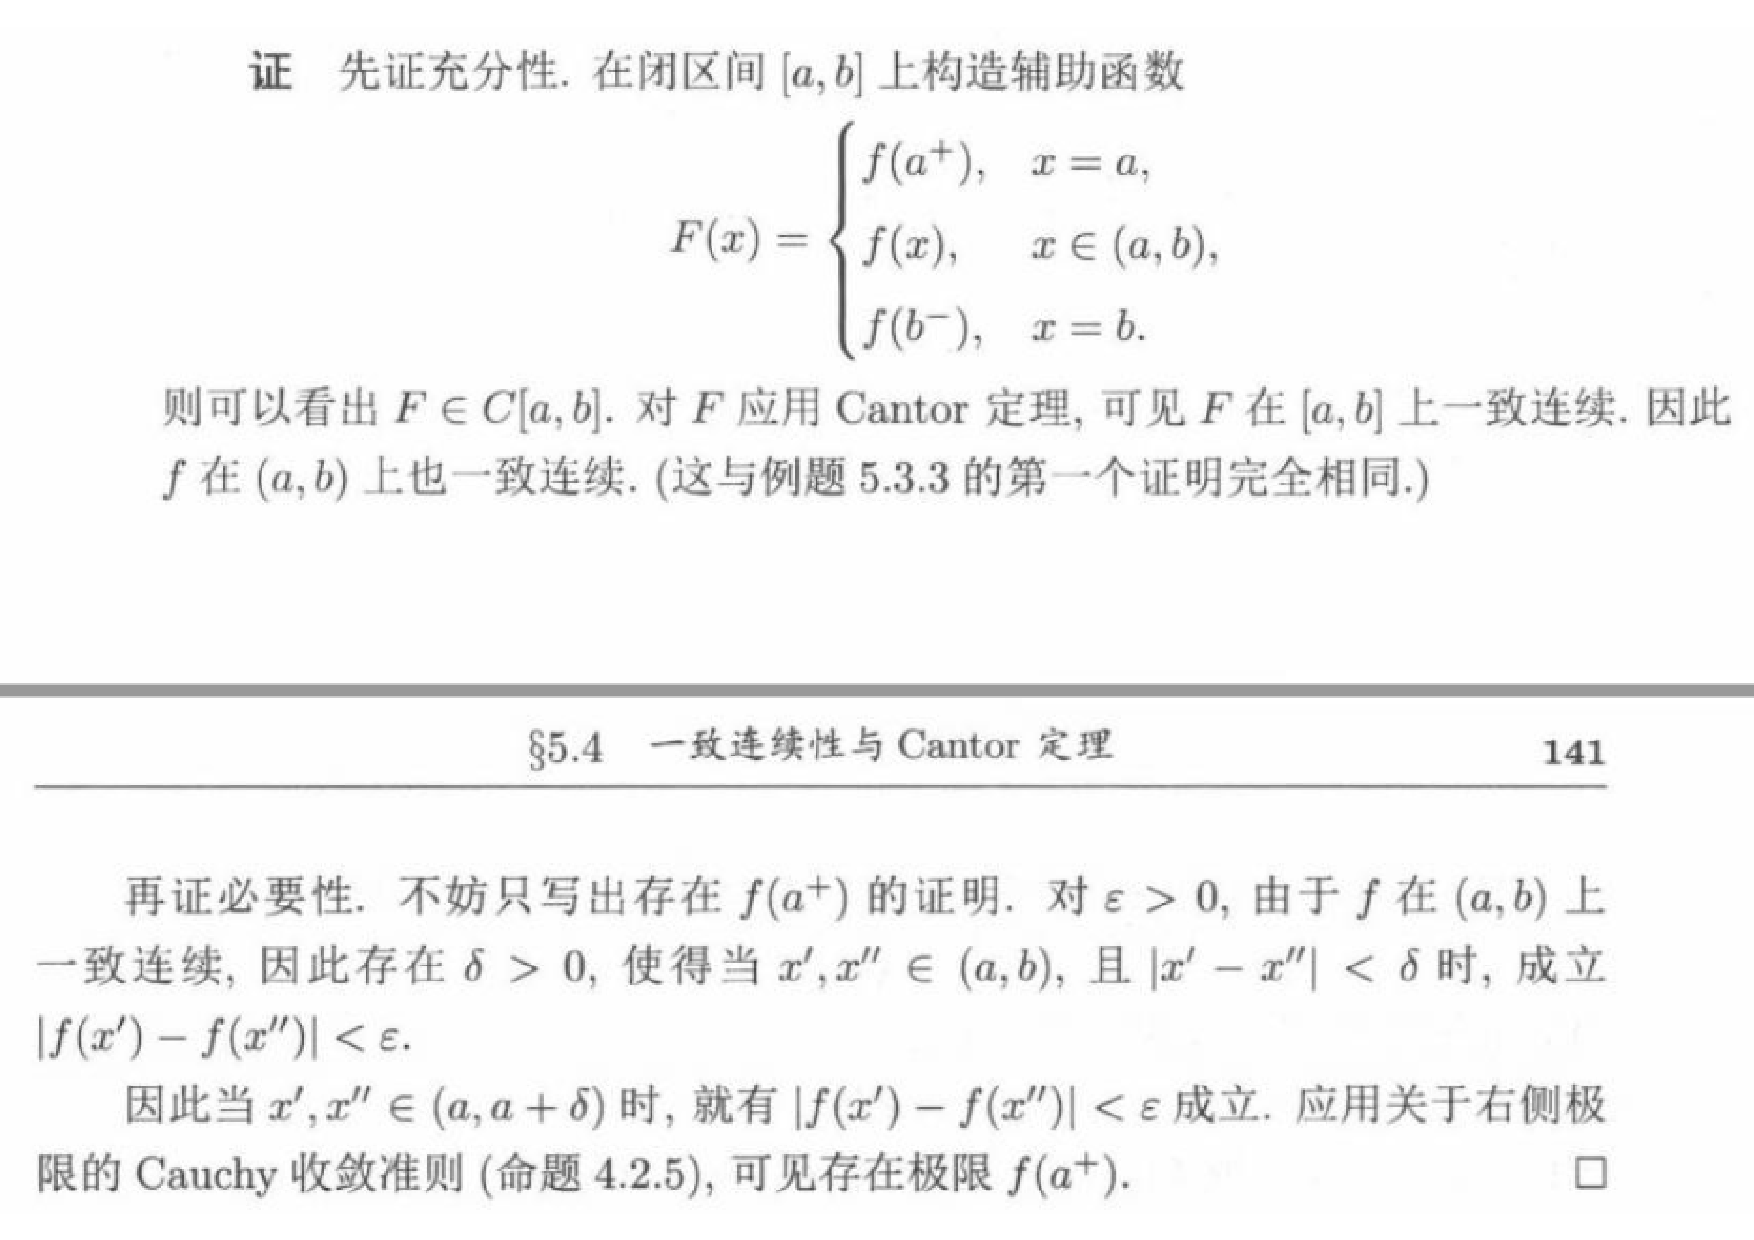
\includegraphics[scale=0.5]{Cantor定理在开区间上的推广证明.pdf}
    \end{figure} 
\end{proof}

\begin{proposition}\label{pro:一阶导数可被二阶导数和原函数控制}
    设\(f\)在\([a,b]\)上二阶可微,且\(\vert f(x)\vert\leqslant A\),\(\vert f''(x)\vert\leqslant B\),证明:\(\vert f'(x)\vert\leqslant\frac{2A}{b-a}+\frac{B\left( b-a \right)}{2}\).
\end{proposition}
\begin{note}
    积累这种想法:利用$Taylor$定理将$n$阶可导函数$f(x)$在特殊点处(本题是端点处)的函数值分别在$x$($x$可取到所有能展开的点)处展开,再根据$x$的任意性得到$k(k=0,1,\cdots,n)$阶导数$f^{(k)}(x)$的相关结论.
\end{note}
\begin{proof}
    (将\(f(a)\)和\(f(b)\)分别在\(x\)点处展开)由\(Taylor\)定理可知,对\(\forall x\in (a,b)\),\(\exists \xi \in (a,x)\),\(\eta \in (x,b)\),使得
    \begin{align*}
        f(a) = f(x) + f^{\prime}(x)(a - x) + \frac{f^{\prime\prime}(\xi)}{2}(a - x)^2,
f(b) = f(x) + f^{\prime}(x)(b - x) + \frac{f^{\prime\prime}(\eta)}{2}(b - x)^2.
    \end{align*}
上述两式相减得
\begin{align}\label{eq:1.7(展开后相减得到的式子)}
    f(b) - f(a) = f^{\prime}(x)(b - a) + \frac{f^{\prime\prime}(\eta)}{2}(b - x)^2 - \frac{f^{\prime\prime}(\xi)}{2}(a - x)^2.
\end{align}
从而结合\(\vert f(x)\vert\leqslant A\),\(\vert f^{\prime\prime}(x)\vert\leqslant B\),对\(\forall x\in (a,b)\)有
\begin{align*}
    \vert f^{\prime}(x)\vert\leqslant \left\vert\frac{f(b) - f(a)}{b - a}\right\vert + \left\vert\frac{f^{\prime\prime}(\xi)(a - x)^2 - f^{\prime\prime}(\eta)(b - x)^2}{2(b - a)}\right\vert\leqslant \frac{2A}{b - a} + \frac{B}{2(b - a)}[(a - x)^2 + (b - x)^2].
\end{align*}
又根据抛物线的性质易知\((a - x)^2 + (b - x)^2 < (b - a)^2\),\(x\in (a,b)\).代入到上式有
\begin{align*}
   \vert f^{\prime}(x)\vert < \frac{2A}{b - a} + \frac{B(b - a)}{2}.
\end{align*}
最后再结合\(f^{\prime}(x)\)的连续性,可知对\(\forall x\in [a,b]\),均有\(\vert f^{\prime}(x)\vert\leqslant \frac{2A}{b - a} + \frac{B(b - a)}{2}\).

(\(\vert f^{\prime}(a)\vert \xlongequal{f^{\prime}(x)\text{的连续性}}\lim_{x\rightarrow a^+}\vert f^{\prime}(x)\vert \stackrel{\text{极限保不等式性}}{\leqslant} \frac{2A}{b - a} + \frac{B(b - a)}{2}\),\(\vert f^{\prime}(b)\vert\)同理) 
\end{proof}
\begin{remark}
    \hyperref[pro:一阶导数可被二阶导数和原函数控制]{上述命题}中将\(\vert f(x)\vert\)的条件改为\(f(a)=f(b)\),可以得到下面的推论.
\end{remark}

\begin{corollary}\label{pro:一阶导数可被二阶导数和原函数控制(端点函数值相同的情形)}
    设\(f\)在\([a,b]\)上二阶可微,且\(f(a)=f(b)\),\(\vert f''(x)\vert\leqslant B\),证明:\(\vert f'(x)\vert\leqslant\frac{B\left( b-a \right)}{2}\).
\end{corollary}
\begin{proof}
    只需将\eqref{eq:1.7(展开后相减得到的式子)}式改为
    \begin{align*}
        f^{\prime}(x)(b-a)+\frac{f^{\prime\prime}(\eta )}{2}(b-x)^2-\frac{f^{\prime\prime}(\xi )}{2}(a-x)^2=0.
    \end{align*}
    再根据\hyperref[pro:一阶导数可被二阶导数和原函数控制]{上述命题}同理证明,就可以得到\(\vert f'(x)\vert\leqslant\frac{B\left( b-a \right)}{2}\).
\end{proof}

\begin{proposition}\label{pro:Lagrange中值定理的推广(二阶导数)}
    设\(f\)在\([a,b]\)上可微,在\((a,b)\)上二阶可微,证明:存在\(\xi\in(a,b)\),使成立
    \[
    f'(b) - f'(a) = f''(\xi)(b - a).
    \]
    (注意:这里没有假定\(f'\in C[a,b]\))
\end{proposition}
\begin{note}
    (1)因为本题没有假定\(f'\in C[a,b]\),所以不能直接使用各种中值定理证明中值点的存在性(也就不能使用$K$值法构造辅助函数证明).因此只能利用反证法,假设不存在中值点,再构造辅助函数(构造辅助函数的方法见下述(2)),然后分析函数的性态找到矛盾.

    (2)这类中值问题因为条件不够,导致无法使用各种中值定理的问题,所以不能通过\hyperlink{a}{$K$值法}或\hyperlink{a}{解微分方程法}构造辅助函数.而这类问题构造辅助函数的想法实际上与证明$Lagrange$中值定理中构造辅助函数的想法类似.构造的辅助函数$g(x)$需要满足:$g(a)=g(b)=C$($C$为某已知常数),且$g'(\xi)=0$恰好就是需要证明的等式或者$g'(a)=g'(b)=C$($C$为某已知常数),且$g''(\xi)=0$恰好就是需要证明的等式.(构造的辅助函数具体形式一般就两种,见\hyperref[cor:Lagrange中值定理的推广(k+1阶导数)]{推论}中的$g_1(x),g_2(x)$)

    (3)也可以构造$g\left( x \right) =f'\left( x \right) -\frac{f'\left( b \right) -f'\left( a \right)}{b-a}\left( x-a \right)$作为辅助函数,此时有$g(a)=g(b)=f'(a)$,然后同理进行证明$g'(x)=f^{\prime\prime}(x) - \frac{f^{\prime}(b) - f^{\prime}(a)}{b - a}$即可.
\end{note}
\begin{remark}
    记忆这种构造辅助函数的方式.
\end{remark}
\begin{proof}\label{proof:Lagrange中值定理的推广(二阶导数)-证明}
    令\(g(x) = f(x) - \frac{f^{\prime}(b) - f^{\prime}(a)}{b - a} \cdot \frac{(x - a)^2}{2}\),则\(g^{\prime}(x) = f^{\prime}(x) - \frac{f^{\prime}(b) - f^{\prime}(a)}{b - a}(x - a)\),且\(g^{\prime}(a) = g^{\prime}(b) = f^{\prime}(a)\).

(因为只有\(g\in D(a,b)\),而\(g\)不一定在\(a\)、\(b\)处连续,所以不能使用\(Rolle\)中值定理直接得到\(g^{\prime\prime}(\xi) = 0\))

(反证)假设\(g^{\prime\prime}(x) > 0\)或\(g^{\prime\prime}(x) < 0\),\(\forall x\in (a,b)\).当\(g^{\prime\prime}(x) > 0\)时,对\(\forall x\in (a,b)\),有\(f^{\prime}(x)\)在\((a,b)\)上严格递增.
任取\(c\in (a,b)\),则\(f^{\prime}(c) > f^{\prime}(a) = f^{\prime}(b)\).又由\(Darboux\)定理可知,存在\(d\in (c,b)\),使得\(f^{\prime}(c) > f^{\prime}(d) > f^{\prime}(b)\).这与\(f^{\prime}(x)\)在\((a,b)\)上严格递增矛盾.
于是\(g^{\prime\prime}(x) > 0\),对\(\forall x\in (a,b)\)不成立.同理可得\(g^{\prime\prime}(x) < 0\),对\(\forall x\in (a,b)\)也不成立.故一定存在\(\xi \in (a,b)\),使得\(g^{\prime\prime}(\xi) = 0\).

又因为\(g^{\prime\prime}(x) = f^{\prime\prime}(x) - \frac{f^{\prime}(b) - f^{\prime}(a)}{b - a}\),所以\(f^{\prime\prime}(\xi) = \frac{f^{\prime}(b) - f^{\prime}(a)}{b - a}\).即\(f^{\prime}(b) - f^{\prime}(a) = f^{\prime\prime}(\xi)(b - a)\).
\end{proof}
\begin{remark}
    将上述命题推广可以得到下面一个命题.
\end{remark}
\begin{corollary}\label{cor:Lagrange中值定理的推广(k+1阶导数)}
    设\(f\in D^{k}[a,b]\cap D^{k+1}\left( a,b \right) \),则存在\(\xi\in(a,b)\),使成立
    \[
    f^{(k)}(b) - f^{(k)}(a) = f^{(k+1)}(\xi)(b - a).
    \]
\end{corollary}
\begin{note}
    记忆这个推论构造辅助函数的方式以及这个推论的结论.
\end{note}
\begin{proof}
    证明这个命题只需要构造辅助函数$\boldsymbol{g}_{\boldsymbol{1}}\left( \boldsymbol{x} \right) =\boldsymbol{f}\left( \boldsymbol{x} \right) -\frac{\boldsymbol{f}^{\left( \boldsymbol{k} \right)}\left( \boldsymbol{b} \right) -\boldsymbol{f}^{\left( \boldsymbol{k} \right)}\left( \boldsymbol{a} \right)}{\boldsymbol{b}-\boldsymbol{a}}\cdot \frac{\left( \boldsymbol{x}-\boldsymbol{a} \right) ^{\boldsymbol{k}}}{\boldsymbol{k}!}$,则有${g_1}^{\left( k \right)}\left( a \right) ={g_1}^{\left( k \right)}\left( b \right) =f^{\left( k \right)}\left( a \right) .$然后只需要仿造\hyperref[proof:Lagrange中值定理的推广(二阶导数)-证明]{上一个命题的证明}:存在$\xi \in (a,b)$,使得${g_1}^{\left( k+1 \right)}\left( \xi \right) =f^{\left( k+1 \right)}\left( \xi \right) -\frac{f^{\left( k \right)}\left( b \right) -f^{\left( k \right)}\left( a \right)}{b-a}=0$即可.

或者构造辅助函数$\boldsymbol{g}_{\boldsymbol{2}}\left( \boldsymbol{x} \right) =\boldsymbol{f}^{\left( \boldsymbol{k} \right)}\left( \boldsymbol{x} \right) -\frac{\boldsymbol{f}^{\left( \boldsymbol{k} \right)}\left( \boldsymbol{b} \right) -\boldsymbol{f}^{\left( \boldsymbol{k} \right)}\left( \boldsymbol{a} \right)}{\boldsymbol{b}-\boldsymbol{a}}\left( \boldsymbol{x}-\boldsymbol{a} \right)$.则有${g_2}^{\left( k \right)}\left( a \right) ={g_2}^{\left( k \right)}\left( b \right) =f^{\left( k \right)}\left( a \right) .$然后只需要\hyperref[proof:Lagrange中值定理的推广(二阶导数)-证明]{同理证明}:存在$\xi \in (a,b)$,使得$g_2\left( \xi \right) =f^{\left( k+1 \right)}\left( \xi \right) -\frac{f^{\left( k \right)}\left( b \right) -f^{\left( k \right)}\left( a \right)}{b-a}=0$即可.
\end{proof}

\begin{proposition}\label{pro:二阶导数零点的存在性}
    设\(f\)在\((-\infty,+\infty)\)上二阶可微,且有界,证明:存在\(\xi\),使成立\(f''(\xi)=0\).
\end{proposition}
\begin{note}
    当$f''(x)>0$时,$f(x)$是下凸函数,在$(-\infty,+\infty)$上一定会发散到无穷.(即$f(x)$的增速越来越快,不会出现类似$arctanx$那种情况)
\end{note}
\begin{remark}
    如果$f\in D(-\infty,+\infty)$,且有界.那么得不到$f'(x)$在$(-\infty,+\infty)$上有零点.(例如,$f(x)=arctanx$)
\end{remark}
\begin{proof}
    (反证)假设结论不成立,则$f''(x)>0$或$f''(x)<0$恒成立.不妨设$f''(x)>0,x\in (-\infty,+\infty)$.则$f'(x)$在$\mathbb{R}$上严格单调递增.若$f'(0)\ge0$,则对$\forall a>1$,都有$f'(a)>f'(1)>f'(0)\ge0$.从而对$\forall x>1$,根据$Lagrange$中值定理,可知,存在$\eta \in (1,x)$,使得
    \begin{align*}
        f(x)-f(0)=f'(\eta)(x-1)>f'(1)(x-1).
    \end{align*}
    令$x\to +\infty$,得$f(x)\to +\infty$.这与$f(x)$有界矛盾.同理$f'(0)<0$也不成立.于是假设不成立,命题即证.
\end{proof}

\begin{proposition}\label{pro:分式不等式等价变形}
    若\(x_1,x_2,a_1,a_2,b_1,b_2\in \mathbb{R}\),且\(x_2 - a_2 > 0\),\(b_2 - a_2 > 0\),则\(\frac{x_1 - a_1}{x_2 - a_2} < \frac{b_1 - a_1}{b_2 - a_2} \Leftrightarrow \frac{x_1 - a_1}{x_2 - a_2} < \frac{b_1 - x_1}{b_2 - x_2}\).
\end{proposition}
\begin{proof}
    \begin{align*}
        &\,\,\,\,\,\,\,\,\,\,\frac{x_1-a_1}{x_2-a_2}<\frac{b_1-a_1}{b_2-a_2}
        \\
        &\Leftrightarrow \left( x_1-a_1 \right) \left( b_2-a_2 \right) <\left( b_1-a_1 \right) \left( x_2-a_2 \right) 
\\
&\Leftrightarrow \left( x_1-a_1 \right) \left( b_2-x_2+x_2-a_2 \right) <\left( b_1-a_1 \right) \left( x_2-a_2 \right) 
\\
&\Leftrightarrow \left( x_1-a_1 \right) \left( b_2-x_2 \right) +\left( x_1-a_1 \right) \left( x_2-a_2 \right) <\left( b_1-a_1 \right) \left( x_2-a_2 \right) 
\\
&\Leftrightarrow \left( x_1-a_1 \right) \left( b_2-x_2 \right) <\left( b_1-a_1+a_1-x_1 \right) \left( x_2-a_2 \right) 
\\
&\Leftrightarrow \left( x_1-a_1 \right) \left( b_2-x_2 \right) <\left( b_1-x_1 \right) \left( x_2-a_2 \right) 
\\
&\Leftrightarrow \frac{x_1-a_1}{x_2-a_2}<\frac{b_1-x_1}{b_2-x_2}
    \end{align*}
\end{proof}

\section{例题}

\begin{example}\label{example:1.1(由原函数和二阶导数上确界估计一阶导数上确界)}
    设\(f\)在\((0,+\infty)\)上二阶可微,且已知
    \begin{equation}
    M_0=\sup\{\vert f(x)\vert\mid x\in(0,+\infty)\}\text{和}M_2=\sup\{\vert f''(x)\vert\mid x\in(0,+\infty)\}
        \nonumber
    \end{equation}
    为有限数.证明:\(M_1=\sup\{\vert f'(x)\vert\mid x\in(0,+\infty)\}\)也是有限数,并满足不等式
    \begin{equation}
        M_1\leq2\sqrt{M_0M_2}.
        \nonumber
    \end{equation}
        \begin{proof}
        $\forall x,t>0$,由于$f$在$(0,+\infty)$上二阶可微,根据$Taylor$定理,将$f(x+t)$在$x$处展开得,存在$\xi\in(x,x+t)$,使得
        \begin{equation}
    f(x+t)=f(x)+f'(x)t+\frac{f''(\xi)}{2}t^2
    \nonumber
        \end{equation}
        由此有估计
        \begin{equation}
        |tf'(x)|=|f(x+t)-f(x)-\frac{f''(\xi)}{2}t^2|\leqslant2M_0+\frac{M_2}{2}t^2
            \nonumber
        \end{equation}
        这样就得到
        \begin{equation}
    |f'(x)|\leqslant\frac{2M_0}{t}+\frac{M_2}{2}t
            \nonumber
        \end{equation}
        这对每个$x,t\in(0,+\infty)$都成立.
        两边对$x$取上确界,就有
        \begin{equation}
            M_1\leqslant\frac{2M_0}{t}+\frac{M_2}{2}t
            \nonumber
        \end{equation}
        这对每个$t\in(0,+\infty)$都成立.因此,$M_1$为有限数.为了得到最好的估计,
        可以取$t=2\sqrt{\frac{M_0}{M_2}}$,使右边和达到最小,即有
        \begin{equation}
            M_1\leqslant2\sqrt{M_0M_2}.
            \nonumber
        \end{equation}
        \end{proof}
\end{example}
\begin{remark}
    将\hyperref[example:1.1(由原函数和二阶导数上确界估计一阶导数上确界)]{上述例题}中的区间从$(0,+\infty)$改为$(-\infty,+\infty)$.可以得到更好的估计$M_1\leqslant \sqrt{M_0M_2}$.即\hyperref[example:1.1(由原函数和二阶导数上确界估计一阶导数上确界)(区间为R)]{下面一个例题}.
\end{remark}
\begin{example}\label{example:1.1(由原函数和二阶导数上确界估计一阶导数上确界)(区间为R)}
    设\(f\)在\((-\infty,+\infty)\)上二阶可微,且已知
    \begin{equation}
    M_0=\sup\{\vert f(x)\vert\mid x\in(0,+\infty)\}\text{和}M_2=\sup\{\vert f''(x)\vert\mid x\in(0,+\infty)\}
        \nonumber
    \end{equation}
    为有限数.证明:\(M_1=\sup\{\vert f'(x)\vert\mid x\in(0,+\infty)\}\)也是有限数,并满足不等式
    \begin{equation}
        M_1\leq\sqrt{2M_0M_2}.
        \nonumber
    \end{equation}
\end{example}
\begin{proof}
    由于\(f\in D^2(-\infty,+\infty)\),对\(\forall x\in (-\infty,+\infty)\),\(t > 0\),根据\(Taylor\)中值定理,分别将\(f(x + t)\),\(f(x - t)\)在\(x\)处展开可得,存在\(\xi_1\in (x - t,x)\),\(\xi_2\in (x,x + t)\),使得
    \begin{align*}
    f(x - t) = f(x) + f^{\prime}(x)(-t) + \frac{f^{\prime\prime}(\xi_1)}{2}(-t)^2,
f(x + t) = f(x) + f^{\prime}(x)t + \frac{f^{\prime\prime}(\xi_2)}{2}t^2.
    \end{align*}
上面两式相减,可得
\begin{align*}
   f(x + t) - f(x - t) = 2tf^{\prime}(x) + \frac{f^{\prime\prime}(\xi_2)}{2}t^2 - \frac{f^{\prime\prime}(\xi_1)}{2}t^2.
\end{align*}
从而\(f^{\prime}(x) = \frac{f(x + t) - f(x - t)}{2t} + \frac{t[f^{\prime\prime}(\xi_1) - f^{\prime\prime}(\xi_2)]}{4}\).于是
\begin{align*}
    \vert f^{\prime}(x)\vert\leqslant \frac{\vert f(x + t) - f(x - t)\vert}{2t} + \frac{\vert t[f^{\prime\prime}(\xi_1) - f^{\prime\prime}(\xi_2)]\vert}{4}\leqslant \frac{M_0}{t} + \frac{tM_2}{2}.
\end{align*}
上式对\(\forall x\in (-\infty,+\infty)\),\(t > 0\)都成立,并且上式右边与\(x\)无关.两边同时对\(x\)取上确界,就有
\begin{align*}
    M_1\leqslant \frac{M_0}{t} + \frac{tM_2}{2}.
\end{align*}
这对每个\(t > 0\)都成立.取\(t = \sqrt{\frac{2M_0}{M_2}}\),则有
\begin{align*}
    M_1\leqslant \sqrt{2M_0M_2}.
\end{align*} 
\end{proof}
\begin{remark}
    取\(t = \sqrt{\frac{2M_0}{M_2}}\),此时有\(g(t) = \frac{M_0}{t} + \frac{tM_2}{2}\)恰好达到最大值.因此\(M_1\leqslant \sqrt{2M_0M_2}\)是最佳估计.
\end{remark}

\begin{example}
    设\(f\)在\([a,b]\)上二阶可微.证明:存在\(\xi\in(a,b)\),使得
    \begin{equation}
        f(a)-2f\left(\frac{a + b}{2}\right)+f(b)=\frac{1}{4}(b - a)^{2}f^{\prime\prime}(\xi).
        \nonumber
    \end{equation}
    \begin{proof}
        {\color{blue} \text{证法一}}:写出$f(a),f(b)$在点$\frac{a+b}{2}$处的$Taylor$展开式:
        \begin{gather}
            f(a)=f\left( \frac{a+b}{2} \right) +f^{\prime}\left( \frac{a+b}{2} \right) \left( \frac{a-b}{2} \right) +\frac{1}{2}f^{\prime\prime}(\eta _1)\left( \frac{b-a}{2} \right) ^2,\eta _1\in \left( a,\frac{a+b}{2} \right) 
            \nonumber\\
f(b)=f\left( \frac{a+b}{2} \right) +f^{\prime}\left( \frac{a+b}{2} \right) \left( \frac{b-a}{2} \right) +\frac{1}{2}f^{\prime\prime}(\eta _2)\left( \frac{b-a}{2} \right) ^2,\eta _2\in \left( \frac{a+b}{2},b \right) 
            \nonumber
        \end{gather}
        然后将两式相加,就有
        \begin{equation}\label{eq:2..2}
            f\left( a \right) -2f\left( \frac{a+b}{2} \right) +f\left( b \right) =\frac{1}{8}\left( b-a \right) ^2\left[ f^{\prime\prime}\left( \eta _1 \right) +f^{\prime\prime}\left( \eta _2 \right) \right]
            % \nonumber
        \end{equation}
        又$\min \left\{ f^{\prime\prime}\left( \eta _1 \right) ,f^{\prime\prime}\left( \eta _2 \right) \right\} \le \frac{1}{2}\left[ f^{\prime\prime}\left( \eta _1 \right) +f^{\prime\prime}\left( \eta _2 \right) \right] \le \max \left\{ f^{\prime\prime}\left( \eta _1 \right) ,f^{\prime\prime}\left( \eta _2 \right) \right\}$,
        故由$Darboux$定理(定理\ref{Darboux定理})可知,存在$\xi\in\left( \min \left\{ \eta _1,\eta _2 \right\} ,\max \left\{ \eta _1,\eta _2 \right\} \right)$,使得
        \begin{equation}
            f^{\prime\prime}\left( \xi \right) =\frac{1}{2}\left[ f^{\prime\prime}\left( \eta _1 \right) +f^{\prime\prime}\left( \eta _2 \right) \right]
            \nonumber
        \end{equation}
        再结合\eqref{eq:2..2}可得
        \begin{equation}
            f(a)-2f\left(\frac{a + b}{2}\right)+f(b)=\frac{1}{4}(b - a)^{2}f^{\prime\prime}(\xi).
            \nonumber
        \end{equation}

        {\color{blue} \text{证法二(}K\text{值法构造辅助函数)}}:
        记常数$\lambda=\frac{4\left[ f\left( a \right) +f\left( b \right) -2f\left( \frac{a+b}{2} \right) \right]}{\left( b-a \right) ^2}$,
        令
        \begin{equation}
             F\left( t \right) =f\left( t \right) +f\left( a \right) -2f\left( \frac{t+a}{2} \right) -\lambda \frac{\left( t-a \right) ^2}{4}
             \nonumber
        \end{equation}
       则$F(b)=F(a)=0$.由$Rolle$中值定理可知,存在$\eta\in(a,b)$,
       使得$F'(\eta)=0$,即
       \begin{equation}\label{eq:2..3}
        f'\left( \eta \right) -f'\left( \frac{\eta +a}{2} \right) =\frac{\lambda}{2}\left( \eta -a \right)
        % \nonumber
       \end{equation}
       而由$Lagrange$中值定理可知,存在$\xi\in(\frac{\eta +a}{2},\eta)$,使得
       \begin{equation}
        f'\left( \eta \right) -f'\left( \frac{\eta +a}{2} \right) =\frac{f''\left( \xi \right)}{2}\left( \eta -a \right)
        \nonumber
       \end{equation}
       将其代入\eqref{eq:2..3}式可得,$\left[ \frac{f''\left( \xi \right)}{2}-\frac{\lambda}{2} \right] \left( \eta -a \right) =0$.
       从而$\lambda=f''(\xi)$,即有
       \begin{equation}
        f(a)-2f\left(\frac{a + b}{2}\right)+f(b)=\frac{1}{4}(b - a)^{2}f^{\prime\prime}(\xi).
        \nonumber
       \end{equation}
       
        \begin{remark}
            K值法构造辅助函数:首先令$\lambda=f''(\xi)$,代入
            \begin{equation}
                f(a)-2f\left(\frac{a + b}{2}\right)+f(b)=\frac{1}{4}(b - a)^{2}f^{\prime\prime}(\xi).
                \nonumber
            \end{equation}
            得$\lambda=\frac{4\left[ f\left( a \right) +f\left( b \right) -2f\left( \frac{a+b}{2} \right) \right]}{\left( b-a \right) ^2}$,
            然后将需要证明的式子全部移到等式左边,将$f''(\xi)$换成$\lambda$,并将式中常数$a$或$b$改为变量$t$即可得到我们需要构造的辅助函数:
            \begin{equation}
                F\left( t \right) =f\left( t \right) +f\left( a \right) -2f\left( \frac{t+a}{2} \right) -\lambda \frac{\left( t-a \right) ^2}{4}
                \nonumber
            \end{equation}
            然后再反复利用$Rolle$中值定理即可得到结论.
        \end{remark}

        {\color{blue} \text{证法三}}:作辅助函数
        \begin{equation}
            \varphi \left( x \right) =f\left( x+\frac{b-a}{2} \right) -f\left( x \right)
        \nonumber
        \end{equation}
        由$Lagrange$中值定理可知,存在$\eta \in \left( a,\frac{a+b}{2} \right)$,使得
        \begin{equation}\label{本页公式eq:2...4}
            \frac{\varphi \left( \frac{a+b}{2} \right) -\varphi \left( a \right)}{\frac{1}{2}\left( b-a \right)}=\varphi '\left( \eta \right) =f'\left( \eta +\frac{b-a}{2} \right) -f'\left( \eta \right) 
        \end{equation}
        再次由$Lagrange$中值定理可知,存在$\xi \in \left( \eta ,\eta +\frac{b-a}{2} \right)$,使得
        \begin{equation}\label{本页公式eq:2..5}
            \frac{f'\left( \eta +\frac{b-a}{2} \right) -f'\left( \eta \right)}{\frac{1}{2}\left( b-a \right)}=f'\left( \xi \right) 
            % \nonumber
        \end{equation}
        结合\eqref{本页公式eq:2...4}\eqref{本页公式eq:2..5}式可得
        \begin{equation}
            f'\left( \xi \right) =\frac{f'\left( \eta +\frac{b-a}{2} \right) -f'\left( \eta \right)}{\frac{1}{2}\left( b-a \right)}=\frac{\varphi '\left( \eta \right)}{\frac{1}{2}\left( b-a \right)}=\frac{\varphi \left( \frac{a+b}{2} \right) -\varphi \left( a \right)}{\frac{1}{4}\left( b-a \right) ^2}=\frac{f\left( b \right) -2f\left( \frac{a+b}{2} \right) +f\left( a \right)}{\frac{1}{4}\left( b-a \right) ^2}
            \nonumber
        \end{equation}
        整理即得结论.

    \end{proof}
\end{example}

\section{练习}

\begin{exercise}
设$f\in C[0,1]$,在$(0,1)$上可微,并且$f(0)=0,f(1)=1$.
又设$k_1,k_2,\cdots,k_n$是满足$k_1+k_2+\cdots+k_n=1$的$n$个正数.
证明:在$(0,1)$中存在$n$个互不相同的数$t_1,t_2,\cdots,t_n$,使得
\begin{equation}
    \frac{k_1}{f^{\prime}\left( t_1 \right)}+\frac{k_2}{f^{\prime}\left( t_2 \right)}+\cdots +\frac{k_n}{f^{\prime}\left( t_n \right)}=1
    \nonumber
\end{equation}

    \begin{proof}
        由介值定理知,可以在$(0,1)$中插入$x_1,x_2,\cdots,x_n-1$,使得
        \begin{equation}
            0=x_0<x_1<x_2<\cdots<x_n-1<x_n=1
            \nonumber
        \end{equation}
        同时满足
    \begin{equation}
        f(x_1)=k_1,f(x_2)=k_1+k_2,\cdots ,f(x_{n-1})=k_1+k_2+\cdots +k_{n-1}
        \nonumber
    \end{equation}
    在区间$(x_{i-1},x_i)$上用拉格朗日中值定理,
    有存在$t_i\in (x_{i-1},x_i)$,使得
    \begin{equation}
        k_i=f(x_{i-1})-f(x-i)=f^{\prime}(t_i)(x_{i-1}-x_i),i=1,2,\cdots,n.
    \nonumber
    \end{equation}
    这样就有
    \begin{equation}
        \frac{k_1}{f^{\prime}\left( t_1 \right)}+\frac{k_2}{f^{\prime}\left( t_2 \right)}+\cdots +\frac{k_n}{f^{\prime}\left( t_n \right)}=
        \left( x_1-x_0 \right) +\left( x_2-x_1 \right) +\cdots +\left( x_n-x_{n-1} \right) =1.
        \nonumber
    \end{equation}
    \end{proof}

\end{exercise}


\begin{exercise}\label{(ex:2.2)}
    用$Rolle$定理解决以下问题(在方程中出现的系数均为实数):

(1)证明:方程$e^x=ax^2+bx+c$的不同实根不多于3个;

(2)证明:方程$4ax^3+3bx^2+2cx=a+b+c$在$(0,1)$内至少有一个根;

(3)若$f\left( x \right) =a_nx^n+a_{n-1}x^{n-1}+\cdots +a_1x+a_0=0$
有$n+1$个(不同)实根,证明:$f(x)\equiv 0$.

(4)若$2a^2\le 5b$,证明:方程$x^5+ax^4+bx^3+cx^2+\mathrm{d}x+e=0$不可能有5个不同的实根.

(5)证明:$Legendre$多项式$P_n\left( x \right) =\frac{1}{2^nn!}\left[ \left( x^2-1 \right) ^n \right] ^{\left( n \right)}$
在(-1,1)内有$n$个不同实根.

(6)证明:$Laguerre$(拉盖尔)多项式$L_n\left( x \right) =e^x\left( x^ne^{-x} \right) ^{\left( n \right)}$有n个不同正根.

\begin{proof}
    (1)(反证法)令$f(x)=e^x-(ax^2+bx+c)$,
    假设原方程在$\mathbb{R}$上有4个不同实根$x_1,x_2,x_3,x_4$,且$x_1<x_2<x_3<x_4$.则
    \begin{equation}
        f(x_1)=f(x_2)=f(x_3)=f(x_4)=0
        \nonumber
    \end{equation}
    由$Rolle$中值定理知,存在$\xi_i\in(x_i,x_{i+1}),i=1,2,3$,使得
    \begin{equation}
        f^{\prime}(\xi_1)=f^{\prime}(\xi_2)=f^{\prime}(\xi_3)=0
        \nonumber
    \end{equation}
    由$Rolle$中值定理知,存在$\eta_i\in(\xi_i,\xi_{i+1}),i=1,2$,使得
    \begin{equation}
        f''(\eta_1)=f''(\eta_2)=0
        \nonumber
    \end{equation}
    由$Rolle$中值定理知,存在$\zeta\in(\eta_1,\eta_2)$,使得
    \begin{equation}
        f'''(\zeta)=e^\zeta=0
        \nonumber
    \end{equation}
    这与$e^x$在$\mathbb{R}$上没有零点矛盾,故原方程的不同实根不多于3个.

    (2)令$f(x)=4ax^4+3bx^3+2cx^2-(a+b+c)x$,则$f(0)=f(1)=0$.
    由$Rolle$中值定理知,存在$\xi\in(0,1)$,使得$f'(\xi)=0$.
    从而$\xi$就是原方程在$(0,1)$的一个根.

    (3)由$Rolle$中值定理知,存在$\xi_i\in(x_i,x_{i+1})$,使得
    \begin{equation}
        f^{\prime}\left( \xi _1 \right) =f^{\prime}\left( \xi _2 \right) =\cdots =f^{\prime}\left( \xi _n \right) =0
        \nonumber
    \end{equation}
    反复利用$Rolle$中值定理,得
    \begin{align}
            &f'\left( x \right) =na_nx^{n-1}+\left( n-1 \right) a_{n-1}x^{n-2}+\cdots +2a_2x+a_1\text{有}n\text{个零点}
            \\
            &f^{''}(x)=n\left( n-1 \right) a_nx^{n-2}+\left( n-1 \right) \left( n-2 \right) a_{n-1}x^{n-3}+\cdots +3\text{!}a_3x+a_2=0\text{有}n-1\text{个零点}
            \\
            &\cdots \cdots \cdots \cdots \nonumber
            \\
            &f^{(n-1)}(x)=n!a_nx+\left( n-1 \right) !a_{n-1}\text{有}2\text{个零点} \label{1.3}
            \\
            &f^{(n)}(x)=a_nn!\text{有}1\text{个零点}
    \end{align}
    从而$a_n=0$,代入\eqref{1.3}得,$a_{n-1}=0$.依次类推可得,$a_n=a_{n-1}=\cdots=a_1=a_0=0$.
    故$f(x)\equiv 0$.

    (4)(反证法)令$f(x)=x^5+ax^4+bx^3+cx^2+\mathrm{d}x+e$.
    假设原方程有5个不同的实根,即$f(x)=0$有5个不同的实根.则反复利用$Rolle$中值定理可得,
    $f'''(x)=60x^2+24ax+6b$有2个不同的实根.
    
    从而$\Delta=(24a)^2-4\times 60\times 6b>0$,这与$2a^2\le 5b$矛盾.
    故原方程不可能有5个不同的实根.

    (5)令$f(x)=\left( x^2-1 \right) ^n$.
    则$f(x)=\left( x-1 \right) ^n\left( x+1 \right) ^n$为$2n$次多项式,
    且$x=\pm1$分别为$f(x)$的$n$重根.

    从而$f'(x)$以$\pm1$为$n-1$重根,且由$Rolle$中值定理知,
    存在$\xi _{1}^{(1)}\in(-1,1)$,使得$f'(\xi _{1}^{(1)})=0$.

    进而$f''(x)$以$\pm1$为$n-2$重根,且由$Rolle$中值定理知,
    存在$\xi _{1}^{(2)}\in(-1,\xi _{1}^{(1)}),\xi _{2}^{(2)}\in(\xi _{1}^{(1)},1)$,
    使得$f''(\xi _{i}^{(2)})=0,i=1,2$.即$f''(x)$在$(-1,1)$存在两个互异的实根.

    重复以上操作$n$次,可得$f^{(n)}(x)$不再以$\pm1$为根,且$f^{(n)}(x)$在(-1,1)内有$n$个互异的实根.

    事实上,可知
    \begin{equation}
        P_n\left( x \right) =\frac{1}{2^nn!}\left[ \left( x^2-1 \right) ^n \right] ^{\left( n \right)}
        =\frac{1}{2^nn!}f^{(n)}(x)
        \nonumber
    \end{equation}
    从而$P_n(x)$在(-1,1)内也有$n$个互异的实根.
    又因为$P_n(x)$为$n$次多项式函数,所以若$P_n(x)$有$n+1$个不同的实根,
    则根据练习\eqref{(ex:2.2)}第(2)题可知,$P_n(x)\equiv 0$矛盾.故$P_n(x)$在(-1,1)内只有$n$个互异的实根.

    (6)令$f\left( x \right) =x^ne^{-x}$,显然$0$是
    $f(x)$的$n$重根.并且
    \begin{gather}
            f'\left( x \right) =\frac{x^n+nx^{n-1}}{e^x}
            \nonumber\\
f''\left( x \right) =\frac{x^n+2nx^{n-1}+n\left( n-1 \right) x^{n-2}}{e^x}
\nonumber\\
\cdots \cdots \cdots \cdots \cdots \cdots 
\nonumber\\
f^{\left( n \right)}\left( x \right) =\frac{P_n\left( x \right)}{e^x},\text{其中}P\left( x \right) \text{是关于}x\text{的}n\text{次多项式}
\nonumber
    \end{gather}
    从而$f^{\left( k \right)}\left( x \right) =\frac{P_{n,k}\left( x \right)}{e^x},\text{其中}P_{n,k}\left( x \right) \text{是关于}x\text{的}n\text{次多项式}$,$k=0,1,\cdots,n$.
    于是
    \begin{equation}
        \underset{x\rightarrow +\infty}{\lim}f^{\left( k \right)}\left( x \right) =\underset{x\rightarrow +\infty}{\lim}\frac{P_{n,k}\left( x \right)}{e^x}=0,k=0,1,\cdots ,n
        \nonumber
    \end{equation}
    又由0是$f$的$n$重根可知,$0$是$f^{\left( k \right)}\left( x \right)$的$n-k$重根,$k=0,1,\cdots,n$.

    由$f\left( 0 \right) =\underset{x\rightarrow +\infty}{\lim}f\left( x \right) =0$及推广的$Rolle$中值定理(定理\ref{the:Rolle中值定理在无限区间上的推广})可得,
    存在$\xi _{1}^{\left( 1 \right)}\in(0,+\infty)$,使得$f'(\xi _{1}^{\left( 1 \right)})=0$.
    
    进而$f'\left( 0 \right) =\underset{x\rightarrow +\infty}{\lim}f'\left( x \right) =f'\left( \xi _{1}^{\left( 1 \right)} \right) =0$,再运用推广的$Rolle$中值定理(定理\ref{the:Rolle中值定理在无限区间上的推广})可得,
    存在$\xi _{1}^{\left( 2 \right)}\in \left( 0,\xi _{1}^{\left( 1 \right)} \right) ,\xi _{2}^{\left( 2 \right)}\in \left( \xi _{1}^{\left( 1 \right)},1 \right) $,
    使得$f''\left( \xi _{1}^{\left( 2 \right)} \right) =f''\left( \xi _{2}^{\left( 2 \right)} \right) =0$.
    即$f''(x)$存在两个不同的正根.

    于是反复利用推广的$Rolle$中值定理(定理\ref{the:Rolle中值定理在无限区间上的推广})可得,
    $f^{(n)}(x)$存在$n$个不同的正根.

\end{proof}
\end{exercise}

\begin{exercise}
    若$f$在$[a,b]$上满足在$Rolle$中值定理中的条件(即$f\in C[a,b]$且$f(a)=f(b)$),
$f'_+(a)f'_-(b)>0$.

证明:$f'(x)=0$在$(a,b)$中至少有两个根.

\begin{proof}
    令$F(x)=f(x)-f(a)$,则$F(a)=F(b)=0$且$F'_+(a)F'_-(b)>0$.不妨设$F'_+(a)>0,F'_-(b)>0$,则由极限的局部保号性知,存在$a<a_1<b_1<b$,使得$F(a_1)>F(a)=0,F(b_1)<F(b)=0$.
    
    从而由介值定理可知,存在$c\in(a_1,b_1)$,使得$F(c)=F(a)=F(b)=0$.

    于是由$Rolle$中值定理可得,存在$x_1\in(a,c),x_2\in(c,b)$,使得$F'(x_1)=F'(x_2)=0$.即$f'(x_1)=f'(x_2)=0$.
    故$f'(x)=0$在$(a,b)$中至少有两个根.
\end{proof}
\end{exercise}

\begin{exercise}
设$f$在$[a,b]$上连续,在$(a,b)$上可微,且有$0<a<b$成立.证明:存在$\xi\in(a,b)$,使
\begin{equation}
  f(b)-f(a)=\ln\frac{b}{a}\cdot\xi f'(\xi).
  \nonumber
\end{equation}
    \begin{proof}
        令$g(x)=\ln x$,则由$Cauchy$中值定理可得,存在$\xi\in(a,b)$,使得
        \begin{equation}
        \frac{f\left( b \right) -f\left( a \right)}{\ln b-\ln a}=\frac{f\left( b \right) -f\left( a \right)}{g\left( b \right) -g\left( a \right)}=\cdot\xi f'\left( \xi \right) 
            \nonumber
        \end{equation}
        整理即得$f\left( b \right) -f\left( a \right) =\ln \frac{b}{a}\cdot\xi f'\left( \xi \right) $
    \end{proof}
\end{exercise}

\begin{exercise}
设\(f\)在\([a,b]\)上可微,证明:存在\(\xi\in(a,b)\),使
\begin{equation}
2\xi[f(b)-f(a)]=(b^{2}-a^{2})f^{\prime}(\xi)
    \nonumber
\end{equation}
(若应用$Cauchy$中值定理,则要讨论其条件不满足的情况.)
\begin{note}
    因为$Cauchy$中值定理(定理\ref{the:2.1})的条件$f^{\prime2}(x)+g^{\prime2}(x)\neq0$对$\forall x\in(a,b)$可能不满足,所以不能直接使用$Cauchy$中值定理证明.但是可以利用$Cauchy$中值定理证明中的思路,构造类似的辅助函数
    \begin{equation}
    F(x)=f(x)-f(a)-\frac{f(b)-f(a)}{g\left( b \right) -g\left( a \right)}\left[ g\left( x \right) -g\left( a \right) \right] 
        \nonumber
    \end{equation}
    使得$F(a)=F(b)=0$,再运用$Rolle$中值定理得到证明.
\end{note}
\begin{proof}
    令
    \begin{equation}
    F(x)=f(x)-f(a)-\frac{f(b)-f(a)}{b^2-a^2}\left[ x^2-a^2 \right]
        \nonumber
    \end{equation}
    则$F(a)=F(b)=0$且$F(x)\in\mathrm{C}^1[a,b]$.从而由$Rolle$中值定理可得,存在$\xi\in(a,b)$,使得$F'(\xi )=f'(\xi )-\frac{2\xi f(b)-f(a)}{b^2-a^2}=0$.整理即得结论.
\end{proof}
\end{exercise}

\begin{exercise}
设\(f,g\)在\([a,b]\)上连续,在\((a,b)\)上可微,且导函数\(g'(x)\)在区间\((a,b)\)中无零点,证明:存在\(\xi\in(a,b)\),使得
\begin{equation}
\frac{f^{\prime}(\xi)}{g^{\prime}(\xi)}=\frac{f(\xi)-f(a)}{g(b)-g(\xi)}
    \nonumber
\end{equation}

\begin{note}
    因为导函数\(g'(x)\)在区间\((a,b)\)中无零点,所以如果存在$\xi\in(a,b)$满足结论,则$g'(\xi)\ne0,g(b)-g(\xi)\ne0$.

    若$g(b)-g(\xi)=0$,则由$Rolle$中值定理可知,存在$\eta\in(\xi,b)$,使得$g'(\eta)=0$.这与\(g'(x)\)在区间\((a,b)\)中无零点矛盾.
    
    因此,要证明的结论等价于:存在$\xi\in(a,b)$,使得
    \begin{equation}
    F'(\xi)=f^{\prime}(\xi )\left[ g(b)-g(\xi ) \right] -g^{\prime}(\xi )\left[ f(\xi )-f(a) \right] =0
        \nonumber
    \end{equation}
    从而只要构造出相应的辅助函数$F(x)$,使得$F(a)=F(b)$且$F'(x)=f^{\prime}(x)\left[ g(b)-g(x) \right] -g^{\prime}(x)\left[ f(x)-f(a) \right] =0$,再利用$Rolle$中值定理即可证明结论.直接观察可得,需要构造的辅助函数为$F(x)=[f(x)-f(a)][g(b)-g(x)]$.再将上述思路严格化即可得证.
\end{note}

    \begin{proof}
    令$F(x)=[f(x)-f(a)][g(b)-g(x)]$,则$F(a)=F(b)$且\(F\)在\([a,b]\)上连续,在\((a,b)\)上可微.由$Rolle$中值定理可得,存在$\xi\in(a,b)$,使得
    \begin{equation}\label{2.6}
    F'(\xi)=f^{\prime}(\xi )\left[ g(b)-g(\xi ) \right] -g^{\prime}(\xi )\left[ f(\xi )-f(a) \right] =0
    \end{equation}
    根据$g'(x)$在区间$(a,b)$中无零点知,$g'(\xi)\ne0,g(b)-g(\xi)\ne0$.若$g(b)-g(\xi)=0$,则由$Rolle$中值定理可知,存在$\eta\in(\xi,b)$,使得$g'(\eta)=0$.这与\(g'(x)\)在区间\((a,b)\)中无零点矛盾.

    因此,由\eqref{2.6}整理可得
    \begin{equation}
\frac{f^{\prime}(\xi)}{g^{\prime}(\xi)}=\frac{f(\xi)-f(a)}{g(b)-g(\xi)}
    \nonumber
\end{equation}
    \end{proof}
\end{exercise}

\begin{exercise}
7. 设\(f(x)\)在\([0,+\infty)\)上可微,且\(0\leqslant f(x)\leqslant\frac{x}{1 + x^2}\).证明:存在\(\xi>0\),使得\(f'(\xi)=\frac{1-\xi^{2}}{(1+\xi^{2})^{2}}\).
    \begin{note}
        注意到,只需要构造出相应的辅助函数$F(x)$,使得$F'(x)=f'(x)-\frac{1-x^{2}}{(1+x^{2})^{2}}$.再利用$Rolle$中值定理即可得到结论.
        运用常数变易法求解一阶常微分方程构造辅助函数:

        考虑微分方程$y'=-\frac{1-x^{2}}{(1+x^{2})^{2}}$,两边同时积分解得$y=\frac{x}{(1-x^2)^2}$.故可构造辅助函数$F(x)=f(x)-\frac{x}{(1-x^2)^2}$.
    \end{note}
    \begin{proof}
        令$F(x)=f(x)-\frac{x}{(1-x^2)^2}$,由条件可知,
        \begin{gather}
            0\le f(0)\le 0,
            \nonumber
            \\
            0\le f(+\infty)\le \lim_{x \to +\infty} \frac{x}{1+x^2} 
            \nonumber
        \end{gather}
        由迫敛性可知,$f(0)=f(+\infty)=0$.从而根据推广的$Rolle$中值定理(定理\ref{the:Rolle中值定理在无限区间上的推广})可得,存在$\xi\in(0,+\infty)$,使得$F'(\xi)=f'(\xi)-\frac{1-x^2}{(1+x^2)^2}=0$.整理即得结论.
    \end{proof}
\end{exercise}

\begin{exercise}
对于

(1)\(f(x)=ax^2 + bx + c(a\neq0)\),

(2)\(f(x)=\frac{1}{x}(x>0)\),

计算在公式\(f(x+\Delta x)-f(x)=f'(x+\theta\Delta x)\Delta x\)中的\(\theta\),并求极限\(\lim\limits_{\Delta x\to0}\theta\).
    \begin{proof}
    (1)代入得
    \begin{equation}
    [a(x+\Delta x)^2+b(x+\Delta x)+c]-(ax^2+bx+c)=[2a(x+\theta \Delta x)+b]\Delta x
        \nonumber
    \end{equation}
    解得$\theta=\frac{1}{2}$.

    (2)代入得
    \begin{equation}
    \frac{1}{x+\Delta x}-\frac{1}{x}=-\frac{\Delta x}{(1+(x+\theta \Delta x)^2)}
        \nonumber
    \end{equation}
    化简可得
    \begin{equation}
    \Delta x\cdot\theta^2+2\theta x-x=0
        \nonumber
    \end{equation}
    令$\Delta x \to 0$,得$\theta=\frac{1}{2}$.
    \end{proof}
\end{exercise}

\begin{exercise}
证明:当\(x\geq0\)时有\(\sqrt{x+1}-\sqrt{x}=\frac{1}{2\sqrt{x+\theta(x)}}\),其中\(\frac{1}{4}\leq\theta(x)\leq\frac{1}{2}\),且具有性质
\begin{equation}
\lim\limits_{x\to0^{+}}\theta(x)=\frac{1}{4},\lim\limits_{x\to+\infty}\theta(x)=\frac{1}{2}
    \nonumber
\end{equation}

    \begin{proof}
    由$Lagrange$中值定理,存在$\theta(x)\in(0,1)$,使得
    \begin{equation}
    \sqrt{x+1}-\sqrt{x}=\frac{1}{2\sqrt{x+\theta(x)}}
        \nonumber
    \end{equation}
    由此得
    \begin{equation}
    2\sqrt{x+\theta(x)}=\frac{1}{\sqrt{x+1}-\sqrt{x}}=\sqrt{x+1}+\sqrt{x}
        \nonumber
    \end{equation}
    进而
    \begin{equation}\label{2.7}
    \begin{split}
    \theta(x)=\frac{1}{4}[\sqrt{x+1}+\sqrt{x}]^2-x
    =\frac{1}{4}+\frac{1}{2}[\sqrt{x(x+1)}-x]
    \end{split}
    \end{equation}
    由于
    \begin{equation}
    \sqrt{x(x+1)}-x=\frac{x}{\sqrt{x(x+1)}+x}\le \frac{x}{\sqrt{x^2}+x}=\frac{1}{2}
    \nonumber
    \end{equation}
    再结合\eqref{2.7}可得,$\frac{1}{4}\le\theta(x)\le\frac{1}{2}$.
    又由\eqref{2.7}直接可得
    \begin{equation}
    \lim_{x \to 0^{+}} =\frac{1}{4},\lim_{x \to +\infty}=\frac{1}{2}
        \nonumber
    \end{equation}
    \end{proof}
\end{exercise}

\begin{exercise}
    设\(f\)在区间\([a,b]\)上可微.证明:若\(f(a)\)是\(f\)的最大值,
    则\(f^{\prime}_{+}(a)\leq0\):若\(f(b)\)是\(f\)的最大值,
    则\(f^{\prime}_{-}(b)\geq0\).
    \begin{proof}
        若\(f(a)\)是\(f\)的最大值,
        则$\forall x\in[a,b]$,有$f(x) \ge f(a)$.从而
        \begin{equation}
            f_{+}^{\prime}(a)=\lim_{x\rightarrow a^+} \frac{f(x)-f(a)}{x-a}\leqslant 0
            \nonumber
        \end{equation}
        若\(f(b)\)是\(f\)的最大值,同理可得
        \begin{equation}
            f_{-}^{\prime}(b)=\lim_{x\rightarrow b^-} \frac{f(x)-f(b)}{x-b}\geqslant 0
            \nonumber
        \end{equation}
    \end{proof}
\end{exercise}

\begin{exercise}
    证明:当且仅当\(\vert x\vert\leq\frac{1}{\sqrt{2}}\)时,成立\(2\arcsin x\equiv\arcsin(2x\sqrt{1 - x^{2}})\).
    \begin{proof}
    令$f(x)=2\arcsin x-\arcsin(2x\sqrt{1 - x^{2}})$,\(\vert x\vert\leq\frac{1}{\sqrt{2}}\).则
    \begin{equation}
        \begin{split}
            f'\left( x \right) =\frac{2}{\sqrt{1-x^2}}-\frac{2\sqrt{1-x^2}-\frac{2x^2}{\sqrt{1-x^2}}}{\sqrt{1-4x^2\left( 1-x^2 \right)}}
            =\frac{2}{\sqrt{1-x^2}}-\frac{2\left( 1-2x^2 \right)}{\sqrt{1-x^2}\sqrt{\left( 2x^2-1 \right) ^2}}=0
        \end{split}
      \nonumber
    \end{equation}
    从而$f(x)\equiv C$(其中$C$为常数).又因为$f(0)=0$,所以$f(x)\equiv0$.
    \end{proof}
\end{exercise}

\begin{exercise}
    设函数\(f\)在区间\(I\)上二阶可微,且\(f''(x)\equiv0\).问:$f$是什么函数?
    \begin{solution}
    $f$为线性函数,理由如下:

    由$f''(x)=0$可知,$f'(x)=C$,其中$C$为常数.任取$x_0\in I$,对$\forall x\in I$,由拉格朗日中值定理可得,
    存在$\xi\in(\min\{x_0,x\},\max\{x_0,x\})$,使得
    \begin{equation}
        f(x)=f'(\xi)(x-x_0)+f(x_0)
        \nonumber
    \end{equation}
    故$f(x)=c(x-x_0)+f(x_0)$,其中$c=f'(\xi)$,$x\in I$
    \end{solution}
\end{exercise}

\begin{exercise}
    证明:在有界开区间\((a,b)\)上无界的可微函数的导数也一定无界.
    \begin{proof}
        假设$\exists M>0$,$\forall x\in(a,b)$,有$|f'(x)|<M$.
        任取$x_0\in(a,b)$,对$\forall x\in(a,b)$.由拉格朗日中值定理可知,
        存在$\xi\in(min\{x_0,x\},\max\{x_0,x\})$,使得
        \begin{equation}
            \begin{split}
                |f(x)|=|f'(\xi )(x-x_0)+f(x_0)|\leqslant M\left( b-a \right) +|f(x_0)|
            \end{split}
            \nonumber
        \end{equation}
        因此,$f(x)$在区间$(a,b)$上有界.这与$f(x)$在有界开区间\((a,b)\)上无界矛盾.
    \end{proof}
\end{exercise}

\begin{exercise}
    设\(f\)在\((0,a)\)上可微,\(f(0^{+}) = +\infty\).证明:\(f^{\prime}(x)\)在点\(x = 0\)的右侧无下界.
    \begin{proof}
    任取$x_0>0$,由\(f(0^{+}) = +\infty\)可知,$\exists 0<\delta<x_0\,\,s.t.\,\,\forall x\in(0,\delta)$,有$f(x)>f(x_0)$.
    
    从而当$x\in(0,\delta)$时,有
    \begin{equation}
        \frac{f(x)-f(x_0)}{x-x_0}<\frac{f(x)-f(x_0)}{-x_0}<0
        \nonumber
    \end{equation}
    令$x\to0^{+}$,则
    \begin{equation}
        f'(x_0)=\underset{x\rightarrow 0^+}{\lim}\frac{f(x)-f(x_0)}{x-x_0}\leqslant \underset{x\rightarrow 0^+}{\lim}\frac{f(x)-f(x_0)}{-x_0}=\frac{f\left( x_0 \right)}{x_0}-\frac{f\left( 0^+ \right)}{x_0}=-\infty 
        \nonumber
    \end{equation}
    故\(f^{\prime}(x)\)在点\(x = 0\)的右侧无下界.
    \end{proof}
\end{exercise}

\begin{exercise}
    设\(f\)在\([a,b]\)上连续,在\((a,b)\)上可微,\(f(a)=f(b)\),但\(f\)不是常值函数.证明:存在\(\xi\in(a,b)\),使\(f^{\prime}(\xi)>0\).
    \begin{proof}
    因为\(f\)不是常值函数,所以存在$c\in(a,b)$,使得$f(c)\ne f(a)$.
    
    若$f(c)>f(a)=f(b)$,则由拉格朗日中值定理可知,存在$\xi\in(a,c)$,使得
    \begin{equation}
        f'\left( \xi \right) =\frac{f\left( c \right) -f\left( a \right)}{c-a}>0
        \nonumber
    \end{equation}
    若$f(c)<f(a)=f(b)$,则由拉格朗日中值定理可知,存在$\eta\in(c,b)$,使得
    \begin{equation}
        f'\left( \eta \right) =\frac{f\left( b \right) -f\left( c \right)}{b-c}>0
        \nonumber
    \end{equation}
    \end{proof}
\end{exercise}

\begin{exercise}
    设\(f\)在\([0,1]\)上连续,在\((0,1)\)上二阶可微,又知连接点\(A(0,f(0))\)和\(B(1,f(1))\)的直线段与曲线\(y = f(x)\)交于点\(C(c,f(c))\),其中\(0<c<1\).证明:在\((0,1)\)内存在一点\(\xi\),使\(f^{\prime\prime}(\xi)=0\).
    \begin{proof}
    令$F(x)=f(x)-[f(1)-f(0)]x-f(0)$,则由条件可知,$F(0)=F(1)=F(c)=0$.
    从而用两次$Roll$中值定理可得,存在$\xi\in(0,1)$,使得$f''(\xi)=0$.
    \end{proof}
\end{exercise}

\begin{exercise}
    设\(f\)在\([a,b]\)上连续,在\((a,b)\)上可微,且\(f^{\prime}(x)\)无零点.证明:存在\(\xi,\eta\in(a,b)\),使得
    \begin{equation}
        \frac{f^{\prime}(\xi)}{f^{\prime}(\eta)}=\frac{e^{b}-e^{a}}{b - a}e^{-\eta}
    \nonumber
    \end{equation}
    \begin{proof}
        {\color{blue} \text{证法一}}:由拉格朗日中值定理可知,存在$\eta\in(a,b)$,使得
    \begin{equation}
        e^{\eta}=\frac{e^b-e^a}{b-a}
        \nonumber
    \end{equation}
    于是取$\xi=\eta\in(a,b)$,则
    \begin{equation}
        \frac{f^{\prime}(\xi )}{f^{\prime}(\eta )}=\frac{e^b-e^a}{b-a}e^{-\eta}=1
        \nonumber
    \end{equation}

    {\color{blue} \text{证法二}}:一方面,由$Lagrange$中值定理可知,存在$\xi \in(a,b)$,使得
    \begin{equation}\label{eq:2.8}
        \frac{f(b)-f\left( a \right)}{\left( b-a \right) \left( e^b-e^a \right)}=\frac{f^{\prime}(\xi )}{e^b-e^a}
        % \nonumber
    \end{equation}
    另一方面,由$Cauchy$中值定理可知,存在$\eta \in(a,b)$,使得
    \begin{equation}\label{eq:2.9}
        \frac{f(b)-f\left( a \right)}{\left( b-a \right) \left( e^b-e^a \right)}=\frac{f^{\prime}(\eta )}{b-a}e^{-\eta}
        % \nonumber
    \end{equation}
    结合\eqref{eq:2.8}\eqref{eq:2.9}整理即得
    \begin{equation}
        \frac{f^{\prime}(\xi )}{f^{\prime}(\eta )}=\frac{e^b-e^a}{b-a}e^{-\eta}
    \end{equation}
    \end{proof}
\end{exercise}

\begin{exercise}
    设\(f\)在\([0,1]\)上连续,在\((0,1)\)上可微,\(f(0)=f(1)=0\),\(f(\frac{1}{2})=1\).
    证明:
    
    (1) 存在\(\eta\in(\frac{1}{2},1)\),使\(f(\eta)=\eta\);
    
    (2) 对任何实数\(\lambda\),存在\(\xi\in(0,\eta)\),使\(f^{\prime}(\xi)-\lambda(f(\xi)-\xi)=1\).
    \begin{proof}
    (1)令$g(x)=f(x)-x$,则$g(\frac{1}{2})=1>0,g(1)=-1<0$.由零点存在定理可知,存在$\eta\in(\frac{1}{2},1)$,使得$g(\eta)=0$.即$f(\eta)=\eta$.

    (2)对$\forall \lambda\in \mathbb{R}$,
    令$F(x)=e^{-\lambda x}[f(x)-x]$,则$F'(x)=\frac{f'(x)-1-\lambda[f(x)-x]}{e^{2\lambda x}}$.由(1)可知,$F(0)=F(\eta)=0$.
    由$Rolle$中值定理可知,存在$\xi\in(0,\eta)$,使得
    \begin{equation}
    F'(\xi)=\frac{f'(\xi)-1-\lambda[f(\xi)-\xi]}{e^{2\lambda \xi}}=0
        \nonumber
    \end{equation}
    从而$f'(\xi)-\lambda(f(\xi)-\xi)=1$.
    \end{proof}
\end{exercise}

\begin{exercise}
设\(f\)为区间\(I\)上的可微函数.证明:\(f^{\prime}\)为\(I\)上的常值函数的充分必要条件是\(f\)为线性函数.
\end{exercise}
\begin{proof}
充分性显然,下证必要性.设$f'(x)\equiv C$,其中$C$为某一常数.
$\forall x\in I$,任取固定点$x_0\in I$,由$Lagrange$中值定理可知,
存在$\xi\in(\min\{x_0,x\},\max\{x_0,x\})$,使得
\begin{align*}
f(x)=f'(\xi)(x-x_0)+f(x_0)=C(x-x_0)+f(x_0).
\end{align*}
故$f(x)$为线性函数.
\end{proof}

\begin{exercise}
    用间接法求函数\(f(x)=\sin x^3\)的带 $Peano$ 余项的 $Maclaurin$ 公式,要求写出直到\(x^{13}\)项的系数然后利用这个公式计算出函数\(f(x)\)在点\(x = 0\)的直到\(13\)阶的各阶导数值.
    \begin{proof}
        \begin{equation}
            \begin{split}
                \sqrt[3]{\sin x^3}&=\left( x^3-\frac{1}{3!}x^9+\frac{1}{5!}x^{15}+o\left( x^{15} \right) \right) ^{\frac{1}{3}}
\\
&=x\left( 1-\frac{1}{3!}x^6+\frac{1}{5!}x^{12}+o\left( x^{12} \right) \right) ^{\frac{1}{3}}
\\
&=x\left[ 1+\frac{1}{3}\left( -\frac{1}{3!}x^6+\frac{1}{5!}x^{12}+o\left( x^{12} \right) \right) -\frac{\frac{1}{3}\cdot \frac{2}{3}\left( -\frac{1}{3!}x^6+\frac{1}{5!}x^{12}+o\left( x^{12} \right) \right) ^2}{2!}+o\left( x^{12} \right) \right] 
\\
&=x\left[ 1-\frac{x^6}{18}+\frac{x^{12}}{360}-\frac{1}{324}x^{12}+o\left( x^{12} \right) \right]\\
&=x-\frac{x^7}{18}-\frac{1}{3240}x^{13}+o\left( x^{13} \right)
            \end{split}
            \nonumber
        \end{equation}
        由$Taylor$展开式的唯一性可知
        \begin{gather}
            f^{\prime}(0)=1,f^{(k)}(0)=0,k=2,3,4,5,6,8,9,10,11,12\nonumber\\
            f^{(7)}(0)=-\frac{1}{18},f^{(13)}(0)=-\frac{1}{3240}\nonumber
        \end{gather}
    \end{proof}
\end{exercise}

\begin{exercise}
   计算\(\arcsin x\)的带 $Peano$ 余项的 $Maclaurin$ 公式.
    \begin{proof}
    由于
    \begin{equation}
    (1+x)^\alpha =1+\sum_{k=0}^{+\infty}\frac{\alpha(\alpha-1)\cdots(\alpha-k+1)}{k!}
        \nonumber
    \end{equation}
    所以令$\alpha=-\frac{1}{2}$,用$-x^2$替换$x$得
    \begin{equation}
    \frac{1}{\sqrt[]{1-x^2} } =1+\sum_{k=1}^{+\infty}\frac{(-1)^k\frac{1}{2}\frac{3}{2}\cdots\frac{2k-1}{2}}{k!}(-x^2)^{k}
    =1+\sum_{k=1}^{+\infty}\frac{1\cdot3\cdots(2k-1)}{2^n\cdot k!}x^{2k}
    =1+\sum_{k=1}^{+\infty}\frac{(2k-1)!!}{(2k)!!}x^{2k}
        \nonumber
    \end{equation}
    从而
    \begin{equation}
    \arcsin x=\int_{0}^{x} \frac{1}{\sqrt{1-t^2}}dt=\int_{0}^{x} [1+\sum_{k=1}^{+\infty}\frac{(2k-1)!!}{(2k)!!}t^{2k}]dt
    =x+\sum_{k=1}^{+\infty}\frac{(2k-1)!!}{(2k)!!(2k+1)}x^{2k+1}
        \nonumber
    \end{equation}
    于是$\arcsin x$带$Peano$余项的$Taylor$展开为:
    \begin{equation}
    \arcsin x==x+\sum_{k=1}^{n}\frac{(2k-1)!!}{(2k)!!(2k+1)}x^{2k+1}+o(x^{2n+1})
        \nonumber
    \end{equation}
    \end{proof}
\end{exercise}

\begin{exercise}
    计算$f(x)=\frac{\arcsin x}{\sqrt{1-x^2}}$的带 $Peano$ 余项的 $Maclaurin$ 公式.
    \begin{proof}
    令\(y=\frac{\arcsin x}{\sqrt{1 - xy}}\),两边对\(x\)求导可得
    \begin{gather}
    \sqrt{1 - x^{2}}y'-\frac{xy}{\sqrt{1 - x^{2}}}=\frac{1}{\sqrt{1-x^2}}
    \nonumber\\
    \text{即}(1 - x^{2})y' = 1 + xy
    \nonumber
    \end{gather}
    显然$y=\frac{\arcsin x}{\sqrt{1 - xy}}$为奇函数,根据$Taylor$定理可知,不妨设\(y=\sum_{n = 0}^{\infty}a_{2n-1}x^{2n-1}\),代入上式,得
    \begin{equation}
    a_{1}+\sum_{n = 1}^{\infty}\left((2n + 1)a_{2n + 1}-(2n - 1)a_{2n - 1}\right)x^{2n}=1+\sum_{n = 1}^{\infty}a_{2n - 1}x^{2n}
    \nonumber
    \end{equation}
    对比系数可得
    \begin{equation}
    \begin{cases}a_{1}=1\\(2n + 1)a_{2n + 1}=2na_{2n}\end{cases}
    \nonumber
    \end{equation}
    于是可得\(a_{2n + 1}=\frac{(2n)!!}{(2n + 1)!!}\),\(n = 0,1,2,\cdots\).
    
    从而\(y=\frac{\arcsin x}{\sqrt{1 - xy}}\)有 $Peano$ 余项的麦克劳林公式为
    \begin{equation}
         f(x)=x+\frac{2}{3}x^{3}+\frac{4!!}{5!!}x^{5}+\cdots+\frac{(2n)!!}{(2n + 1)!!}x^{2n + 1}+o(x^{2n + 1})
        \nonumber
    \end{equation}    
    \end{proof}
\end{exercise}

\begin{exercise}
估计下列近似公式的绝对误差:

(1) \(e^{x}\approx1 + x+\frac{x^{2}}{2!}+\cdots+\frac{x^{n}}{n!}\),当 \(0\leq x\leq1\);

(2)$\sin x\approx x-\frac{x^3}{6},当\|x|\le\frac{1}{2}$;

(3) \(\tan x\approx x+\frac{x^{3}}{3}\),当 \(\vert x\vert\leq\frac{1}{10}\);

(4) \(\sqrt{1 + x}\approx1+\frac{x}{2}-\frac{x^{2}}{8}\),当 \(0\leq x\leq1\).
\begin{proof}
    由带有拉格朗日余项的麦克劳林公式得
    \begin{equation}
    f(x)=f(0)+f^{\prime}(0)x+\frac{f^{\prime\prime}(0)}{2!}x^{2}+\cdots+\frac{f^{(n)}(0)}{n!}x^{n}+\frac{f^{(n + 1)}(\xi)}{(n + 1)!}x^{n + 1}
    \nonumber
    \end{equation}
    可得绝对误差为
    \begin{equation}
        \mathbf{(}1)|R\left( x \right) |==\frac{\vert f^{(n + 1)}(\xi)\vert}{(n + 1)!}\vert x\vert^{n + 1}
        \nonumber
    \end{equation}

        (1)$|R\left( x \right) |=\left| \frac{e^{\xi}}{\left( n+1 \right) !}x^{n+1} \right|\le \frac{e}{\left( n+1 \right) !};$
        
        (2)$|R\left( x \right) |=\left| \frac{\sin \xi}{4!}x^4 \right|\le \frac{1}{4!\cdot 2^4}=\frac{1}{384};$

        (3)$|R\left( x \right) |=\left| \frac{\tan ^{\left( 4 \right)}x}{4!}x^4 \right|\le \left| \frac{\tan ^{\left( 4 \right)}\left( 0.1 \right)}{4!}0.1^4 \right|\approx 0.004286 \left( \left( \tan x \right) ^{\left( 4 \right)}\text{在}\left( -0.1,0.1 \right) \text{上单调递增} \right) ;$
        
        (4)$|R\left( x \right) |\le \frac{\left| f^{\left( 3 \right)}\left( 1 \right) \right|}{3!}\approx 0.011.$
\end{proof}
\end{exercise}

\begin{exercise}
    若函数\(f\)在某点\(x_0\)的任意阶 $Taylor$ 多项式均恒等于\(0\),是否可推出\(f(x)\equiv0\)?(参考例题\(6.2.4\)的结论.
    \begin{solution}
        不能,反例(详细见谢惠民上册P169-170例题6.2.4):
        \begin{equation}
            f\left( x \right) =\begin{cases}
            e^{-\frac{1}{x^2}}&,x\ne 0\\
            0&,x=0\\
        \end{cases}
        ,f^{(n)}(0)=0
        \nonumber
        \end{equation}
        \begin{figure}[htbp]
            \centering
            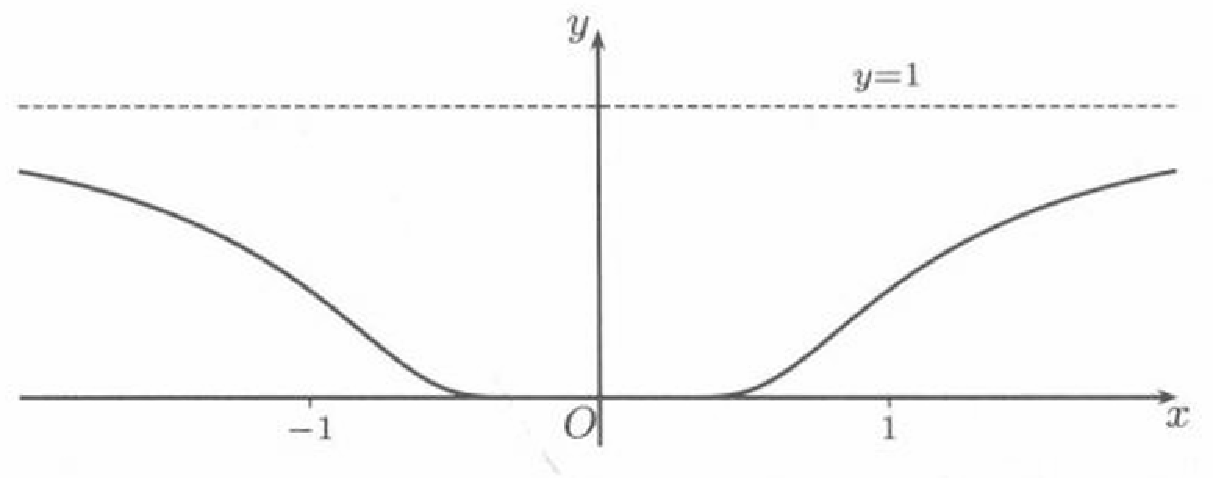
\includegraphics[scale=0.5]{在0点处n阶导数为0的函数图像.pdf}
            % \caption{figure title}
            % \label{figure}
        \end{figure}            
    \end{solution}
\end{exercise}


\begin{exercise}
    设\(f\)在\([-1,1]\)上有任意阶导数,\(f^{(n)}(0)=0\),\(\forall n\in\mathbb{N}_4\),且存在常数\(C\geq0\),使得对所有\(n\in\mathbb{N}^+\)和\(x\in[-1,1]\)成立不等式\(\vert f^{(n)}(x)\vert\leq n!C^{n}\).证明:\(f(x)\equiv0\).
    \begin{proof}
        若$C<1$,则$\forall x\in[-1,1]$,由$Taylor$ 定理可知,存在$\theta_1\in(0,1)$,使得
        \begin{equation}
            \left| f\left( x \right) \right|=\left| \sum_{i=0}^n{\frac{f^{\left( i \right)}\left( 0 \right)}{i!}x^i}+\frac{f^{\left( n+1 \right)}\left( \theta_1 x \right)}{\left( n+1 \right) !}x^{n+1} \right|=\left| \frac{f^{\left( n+1 \right)}\left( \theta_1 x \right)}{\left( n+1 \right) !}x^{n+1} \right|\leqslant C^{n+1}
            \nonumber
        \end{equation}
        上式对任意$n\in\mathbb{N} _+$都成立,
        令$n \to +\infty$,则$f(x)\equiv0$,$\forall x\in[-1,1]$.

        若$C\ge 1$,则对$\forall x\in(-\frac{1}{2C},\frac{1}{2C})$,$\forall k\in \mathbb{N}$,
        根据$Taylor$定理可知,存在$\theta_2\in(0,1)$,使得
        \begin{equation}
            \left| f^{\left( k \right)}\left( x \right) \right|=\left| \sum_{i=k}^{n+k}{\frac{f^{\left( i \right)}\left( 0 \right)}{i!}x^i}+\frac{f^{\left( n+k \right)}\left( \theta_2 x \right)}{\left( n+k \right) !}x^{n+k} \right|=\left| \frac{f^{\left( n+k \right)}\left( \theta_2 x \right)}{\left( n+k \right) !}x^{n+k} \right|\leqslant C^{n+k}\frac{1}{\left( 2C \right) ^{n+k}}=\frac{1}{2^{n+k}}
            \nonumber
        \end{equation}
        上式对任意$n\in\mathbb{N}$都成立,
        令$n\to+\infty$,则$f^{(k)}(x)\equiv0$,$\forall x\in(-\frac{1}{2C},\frac{1}{2C}),\forall k\in \mathbb{N}$.
        根据$f^{(k)}$的连续性可知,$f^{(k)}(-\frac{1}{2C})=f^{(k)}(\frac{1}{2C})=0$.
        故$f^{(k)}(x)\equiv0$,$\forall x\in[-\frac{1}{2C},\frac{1}{2C}],\forall k\in \mathbb{N}$.

        构造数集
        \begin{equation}
            A=\left\{ \alpha \in \left[ -1,0 \right) |f^{\left( n \right)}\left( x \right) \equiv 0,\forall x\in \left[ \alpha ,0 \right] ,\forall n\in \mathbb{N} \right\} ,B=\left\{ \beta \in \left( 0,1 \right] |f^{\left( n \right)}\left( x \right) \equiv 0,\forall x\in \left[ 0,\beta \right] ,\forall n\in \mathbb{N} \right\} 
            \nonumber
        \end{equation}
        显然数集$A,B$有界.根据已证结论可知,$-\frac{1}{2C}\in A,\frac{1}{2C}\in B$,
        故$A,B\ne \varnothing$.
        由确界存在定理可知,数集$A,B$都存在上、下确界.
        设$a=inf\,\,A,b=sup\,\,B$,则根据已证结论可知,$-1\le a<b\le 1$.
        
        我们断言$a\in A,b\in B$,先证$b\in B$.
        由$b=sup\,\,B$可知,对
        $\forall 0<\beta_1<b$,都存在$\beta_1<\beta_0<b$,使得$\beta_0\in B$.
        再根据数集$B$的定义可知,$\beta_1\in B$.
        从而对$\forall 0<\beta_1<b$,都有$f^{\left( k \right)}\left( x \right) \equiv 0,\forall x\in \left[ 0,\beta_1 \right] ,\forall k\in \mathbb{N}$.
        于是对$\forall x\in(0,b)$,都有$f^{(k)}(x)\equiv0,\forall k\in \mathbb{N}$.

        进而,由$f^{(k)}(x),\forall k\in \mathbb{N}$的连续性可知
        \begin{equation}
            f^{\left( k \right)}\left( b \right) =\underset{x\rightarrow b^-}{\lim}f\left( x \right) =0,\forall k\in \mathbb{N}
            \nonumber
        \end{equation}
        因此,$\forall x\in(0,b]$,都有$f^{(k)}(x)\equiv0,\forall k\in\mathbb{N}$.
        故$b\in B$,同理可证$a\in A$.

        我们再断言必有$a=-1,b=1$.先证$b=1$.若$b<1$,取$\delta=\min \left\{ \frac{1}{2C},1-b \right\}$,
        则$\forall x\in[b,b+\delta],\forall k\in\mathbb{N}$,根据$Taylor$定理可知,存在$\theta_0\in(0,1)$,使得
        \begin{equation}
            \begin{split}
                \left| f^{\left( k \right)}\left( x \right) \right|&=\left| \sum_{i=k}^{n+k}{\frac{f^{\left( i \right)}\left( b \right)}{i!}\left( x-b \right) ^i}+\frac{f^{\left( n+k \right)}\left( b+\theta _0\left( x-b \right) \right)}{\left( n+k \right) !}\left( x-b \right) ^{n+k} \right|
\\
&=\left| \frac{f^{\left( n+k \right)}\left( b+\theta _0\left( x-b \right) \right)}{\left( n+k \right) !}\left( x-b \right) ^{n+k} \right|
\\
&\leqslant C^{n+k}\delta ^{n+k}\leqslant C^{n+k}\frac{1}{\left( 2C \right) ^{n+k}}=\frac{1}{2^{n+k}}
            \end{split}
            \nonumber
        \end{equation}
        上式对任意$n\in\mathbb{N}$都成立,
        令$n \to +\infty$,则$f^{(k)}(x)\equiv0$,$\forall x\in[b,b+\delta]$.
        又因为我们已经证得对$\forall x\in(0,b]$,都有$f^{(k)}(x)\equiv0,\forall k\in\mathbb{N}$,
        所以对$\forall x\in(0,b+\delta]$,都有$f^{(k)}(x)\equiv0,\forall k\in\mathbb{N}$.
        故$b+\delta \in B$,这与$b=sup\,\,B$矛盾.因此,$b=1$.类似可证$a=-1$.
        从而根据数集$A,B$的定义可知
        \begin{equation}
            f^{\left( k \right)}\left( x \right) \equiv 0,\forall x\in \left[ -1,1 \right] ,\forall k\in \mathbb{N} 
            \nonumber
        \end{equation}
        综上可知,$f(x)\equiv0,x\in(-1,1)$.
    \end{proof}
\end{exercise}

\begin{exercise}
    设\(f\)在\([a,b]\)上二阶可微,且\(f^{\prime}(a)=f^{\prime}(b)=0\).证明:存在\(\xi\in(a,b)\),使得成立
    \begin{equation}
        \left| f^{\prime\prime}(\xi ) \right|\ge \frac{4}{(b-a)^2}\left| f(b)-f(a) \right|\
        \nonumber
    \end{equation}
    \begin{note}
    已知插值点条件:$f(a),f(b),f'(a)=f'(b)=0$.
    由插值定理可知,插值多项式为3次,余项为4阶导数.但题目条件只有$f$二阶可微,微分条件不够,因此,需要分段插值(靠近哪边就在哪边插值).又因为没有其它约束条件,所以需要找一个公共点能同时在两边都能插值并且能据此推出结论.(显然这个公共点为$\frac{a+b}{2}$)
\end{note}
\begin{remark}
        $f$关于同一个插值点的不同阶导数运用插值定理得到的多项式实际上就是$f$在该点的$Taylor$展开公式,因此$Taylor$定理实际上就是插值定理的一个特例.
\end{remark}
    \begin{proof}
    {\color{blue} \text{证法一}}:
    根据带$Lagrange$余项的$Taylor$定理,将$f(x)$在$a,b$点处分别展开并代入$x=\frac{a+b}{2}$可知,存在$\xi_1\in(a,\frac{a+b}{2}),\xi_2\in(\frac{a+b}{2},b)$,使得
    \begin{gather}
    f(\frac{a+b}{2})=f(a)+\frac{f''(\xi_1)}{2!}(\frac{b-a}{2})^2
    \nonumber
    \\
    f(\frac{a+b}{2})=f(b)+\frac{f''(\xi_2)}{2!}(\frac{b-a}{2})^2
    \nonumber
    \end{gather}
    两式相减可得
    \begin{equation}
    \frac{4}{(b-a)^2}[f(b)-f(a)]=\frac{f''(\xi_1)-f''(\xi_2)}{2}\leqslant \frac{|f''(\xi_1)|+|f'(\xi_2)|}{2}\leqslant \max\{|f''(\xi_1)|,|f''(\xi_2)|\}
        \nonumber
    \end{equation}
    取$\xi=\xi_i$,其中$|f''(\xi_i)|= \max\{|f''(\xi_1)|,|f''(\xi_2)|\}$,则有
    \begin{equation}
\left| f^{\prime\prime}(\xi ) \right|\ge \frac{4}{(b-a)^2}\left| f(b)-f(a) \right|\
        \nonumber
    \end{equation}
    
    {\color{blue} \text{证法二(插值定理和K值法)}}:
    根据插值定理,$f(x)$分别代入插值点$f(a),f'(a)=0$和$f(b),f'(b)=0$,并代入$x=\frac{a+b}{2}$可知,存在$\xi_1\in(a,\frac{a+b}{2}),\xi_2\in(\frac{a+b}{2},b)$,使得
    \begin{gather}
    f(\frac{a+b}{2})=f(a)+\frac{f''(\xi_1)}{2!}(\frac{b-a}{2})^2
    \nonumber
    \\
    f(\frac{a+b}{2})=f(b)+\frac{f''(\xi_2)}{2!}(\frac{b-a}{2})^2
    \nonumber
    \end{gather}
    两式相减可得
    \begin{equation}
    \frac{4}{(b-a)^2}[f(b)-f(a)]=\frac{f''(\xi_1)-f''(\xi_2)}{2}\leqslant \frac{|f''(\xi_1)|+|f'(\xi_2)|}{2}\leqslant \max\{|f''(\xi_1)|,|f''(\xi_2)|\}
        \nonumber
    \end{equation}
    取$\xi=\xi_i$,其中$|f''(\xi_i)|= \max\{|f''(\xi_1)|,|f''(\xi_2)|\}$,则有
    \begin{equation}
\left| f^{\prime\prime}(\xi ) \right|\ge \frac{4}{(b-a)^2}\left| f(b)-f(a) \right|\
        \nonumber
    \end{equation}
    \end{proof}
\end{exercise}
\begin{exercise}
(1) 设\(f\)在\((a,b)\)上可微.试问对每个点\(\xi\in(a,b)\),是否一定存在两个点\(x_1,x_2\in(a,b)\),使得

\begin{equation}
\frac{f(x_2)-f(x_1)}{x_2 - x_1}=f^{\prime}(\xi)
\nonumber
\end{equation}
(2) 设\(f\)在\((a,b)\)上可微,且在某点\(\xi\in(a,b)\)处有\(f''(\xi)>0\).证明:存在两个点\(x_1,x_2\in(a,b)\),使得成立
\begin{equation}
    \frac{f(x_2)-f(x_1)}{x_2 - x_1}=f^{\prime}(\xi)
    \nonumber
\end{equation}
\begin{note}
    思路分析:
    (2)中要证结论等价于:存在两个点\(x_1,x_2\in(a,b)\),使得成立
    \begin{gather}
         f'(\xi)(x_2-x_1)=f(x_2)-f(x_1)\nonumber
         \\
         \Leftrightarrow f(\xi)(x_2-\xi)-f'(\xi)(x_1-\xi)=f(x_2)-f(x_1)
         \nonumber
         \\
         \Leftrightarrow f(x_1)-f'(\xi)(x_1-\xi)=f(x_2)-f'(\xi)(x_2-\xi)\nonumber
    \end{gather}
    根据题目条件和$Taylor$定理,我们构造辅助函数$F(x)=f(x)-g(x)-\varepsilon=f(x)-f'(\xi)(x-\xi)-f(\xi)-\varepsilon$,则原结论等价于证明:
    存在两个点\(x_1,x_2\in(a,b)\),使得成立$GF(x_1)=F(x_2)=C$,其中$C$某一常数.再根据介值定理或零点存在定理找到符合条件的$x_1,x_2$即可.
\end{note}
    \begin{proof}
        (1)不一定,反例:
        $f(x)=x^3$在$(-1,1)上$.对$\xi=0$,$\forall x_1,x_2\in(-1,1)$,有
        \begin{equation}
        \frac{f(x_2)-f(x_1)}{x_2-x_1}=\frac{x^3_2-x^3_1}{x_2-x_1}>0=f'(\xi)
            \nonumber
        \end{equation}
    
    (2)因为$f''(x)>0$,根据导数定义和极限的局部保号性可知,存在$\delta>0$,使得$\forall x\in(\xi-\delta,\xi)$,有$f'(x)<f'(\xi)$.以及$\forall y\in(\xi,\xi+\delta)$,有$f'(x)>f'(\xi)$.
    在$(\xi-\delta,\xi)$和$(\xi,\xi+\delta)$中任取固定点$x_1$和$y_1$.由Taylor定理,分别将$f(x_1)$和$f(y_1)$在点$\xi$处展开,从而存在$x_0\in(x_1,\xi), y_0\in(\xi,y_1)$,使得
    \begin{gather}
        f(x_1) = f(\xi) + f'(x_0)(x_1 - \xi) \nonumber\\
        f(y_1) = f(\xi) + f'(y_0)(y_1 - \xi) \nonumber
    \end{gather}
    
    令$g(x)=f'(\xi)(x-\xi)+f(\xi)$,则
    \begin{gather}
        f(x_1)-g(x_1)=[f'(x_0)-f'(\xi)](x_1-\xi)>0
        \nonumber
        \\
        f(x_2)-g(x_2)=[f'(y_0)-f'(\xi)](y_1-\xi)>0
        \nonumber
    \end{gather}
    取$\varepsilon=\min\{\frac{f(x_1)-g(x_1)}{2},\frac{f(y_1)-g(y_1)}{2}\}$,令$F(x)=f(x)-g(x)-\varepsilon$,则
    \begin{gather}
    F(x_1)\geqslant \frac{f(x_1)-g(x_1)}{2}>0\nonumber
    \\
    F(y_1)\geqslant \frac{f(y_1)-g(y_1)}{2}>0
    \nonumber \\
    F(\xi)=f(\xi)-\varepsilon=-\varepsilon<0
        \nonumber
    \end{gather}

    根据零点存在定理可知,存在$x_3\in(x_1,\xi),y_3\in(\xi,y_1)$,使得
    \begin{gather}
    F(x_3)=F(y_3)=0
        \nonumber
    \end{gather}
    故
    \begin{equation}
        \begin{split}
        &\,\,\,\,\,\,\,\,\,\,f(x_3)-g(x_3)=f(y_3)-g(y_3)
        \nonumber
        \\
        &\Rightarrow f(x_3)-f(\xi)(x_3-\xi)=f(y_3)-f'(\xi)(y_3-\xi)
        \nonumber
        \\
        &\Rightarrow \frac{f(x_3)-f(y_3)}{x_3 - y_3}=f^{\prime}(\xi)
        \nonumber
    \end{split}
    \end{equation}
    \end{proof}
    \begin{remark}
        用类似的方法可证当$f''(\xi)<0$时命题也是成立的.
    \end{remark}
\end{exercise}

\begin{exercise}
设\(f\)在\([a,+\infty)\)上二阶可微,且\(f(x)\geq0\),\(f^{\prime\prime}(x)\leq0\).证明:在\(x\geq a\)时\(f^{\prime}(x)\geq0\).    
    \begin{proof}
        (反证法)假设存在$x_0\in[a,+\infty)$,使得$f'(x_0)<0$.
        则对$\forall x>x_0$,都有$f(x)<f(x_0)$.
        根据$Taylor$定理可知,对$\forall x>x_1$,都存在$\xi\in(x_0,x)$,使得
        \begin{gather}
            f(x)=f(x_0)+f'(\xi)(x-x_0)\leqslant f(x_0)+f'(x_0)(x-x_0)
            \nonumber
        \end{gather}
        
        任取$x>x_0-\frac{f(x_0)}{f'(x_0)}$,则由上式可知
        \begin{gather}
            f(x)\leqslant f(x_0)+f'(x_0)(x-x_0)<0
            \nonumber
        \end{gather}
        这与$\forall x\in[a,+\infty)$,有$f(x)\ge 0$矛盾.
    \end{proof}
\end{exercise}

\begin{exercise}
    设\(f\)在\((-1,1)\)上\(n + 1\)阶可微,\(f^{(n + 1)}(0)\neq0\),\(n\in\mathbb{N}_+\),在\(0<|x|<1\)上有
    \begin{gather}
        f\left( x \right) =f\left( 0 \right) +f^{\prime}\left( 0 \right) x+\cdots +\frac{f^{\left( n-1 \right)}\left( 0 \right)}{\left( n-1 \right) !}x^{n-1}+\frac{f^{\left( n \right)}\left( \theta x \right)}{n!}x^n,\text{其中}0<\theta <1
        \nonumber
    \end{gather}
    证明:$\lim\limits_{\theta\to0}\theta=\frac{1}{n + 1}$.
\end{exercise}
    \begin{proof}
        根据题设可知
        \begin{gather}
            f\left( x \right) =f\left( 0 \right) +f^{\prime}\left( 0 \right) x+\cdots +\frac{f^{\left( n-1 \right)}\left( 0 \right)}{\left( n-1 \right) !}x^{n-1}+\frac{f^{\left( n \right)}\left( \theta x \right)}{n!}x^n,\text{其中}0<\theta <1
            \nonumber
        \end{gather}
        从而
        \begin{gather}\label{eq:2.15}
            \frac{f^{\left( n \right)}\left( \theta x \right) -f^{\left( n \right)}\left( 0 \right)}{x}=\frac{n!}{x^{n+1}}\left[ f\left( x \right) -f\left( 0 \right) -f^{\prime}\left( 0 \right) x-\cdots -\frac{f^{\left( n-1 \right)}\left( 0 \right)}{\left( n-1 \right) !}x^{n-1}-\frac{x^n}{n!}f^{\left( n \right)}\left( 0 \right) \right] 
            % \nonumber
        \end{gather}
        由带$Peano$余项的$Taylor$展开式可知
        \begin{gather}
            f\left( x \right) =f\left( 0 \right) +f^{\prime}\left( 0 \right) x+\cdots +\frac{f^{\left( n \right)}\left( 0 \right)}{n!}x^n+\frac{f^{\left( n+1 \right)}\left( 0 \right)}{\left( n+1 \right) !}x^{n+1}+o\left( x^{n+1} \right) 
            \nonumber
        \end{gather}
        将其代入\eqref{eq:2.15}式得
        \begin{gather}
            \frac{f^{\left( n \right)}\left( \theta x \right) -f^{\left( n \right)}\left( 0 \right)}{x}=\frac{n!}{x^{n+1}}\left[ \frac{f^{\left( n+1 \right)}\left( 0 \right)}{\left( n+1 \right) !}x^{n+1}+o\left( x^{n+1} \right) \right] =\frac{f^{\left( n+1 \right)}\left( 0 \right)}{n+1}+\frac{n!\cdot o\left( x^{n+1} \right)}{x^{n+1}}
            \nonumber
        \end{gather}
        两边同时令$x\to0$,再结合导数定义可得
        \begin{equation}
        \begin{split}
            f^{\left( n+1 \right)}\left( 0 \right) \cdot \underset{x\rightarrow 0}{\lim}\theta &=\underset{x\rightarrow 0}{\lim}\theta \cdot \frac{f^{\left( n \right)}\left( \theta x \right) -f^{\left( n \right)}\left( 0 \right)}{\theta x}=\underset{x\rightarrow 0}{\lim}\frac{f^{\left( n \right)}\left( \theta x \right) -f^{\left( n \right)}\left( 0 \right)}{x}
            \\
            &=\underset{x\rightarrow 0}{\lim}\left[ \frac{f^{\left( n+1 \right)}\left( 0 \right)}{n+1}+\frac{n!\cdot o\left( x^{n+1} \right)}{x^{n+1}} \right] =\frac{f^{\left( n+1 \right)}\left( 0 \right)}{n+1}
        \end{split}
        \nonumber  
    \end{equation}
        又由于\(f^{(n + 1)}(0)\neq0\),故$\underset{x\rightarrow 0}{\lim}\theta =\frac{1}{n+1}$.
    \end{proof}


\begin{exercise}
    证明:在\(\vert x\vert\leq1\)时存在\(\theta\in(0,1)\),使得\(arcsinx=\frac{x}{\sqrt{1-\left( \theta x \right) ^2}}\),且有\(\lim\limits_{x\to0}\theta=\frac{1}{\sqrt{3}}\).
\end{exercise}
    \begin{proof}
        由$Lagrange$中值定理可得,存在$\theta\in(0,1)$,使得
        \begin{equation}
            \arcsin x-\arcsin 0=\frac{x}{\sqrt{1-\left( \theta x \right) ^2}}
        \nonumber
        \end{equation}
        由上式解得
        \begin{equation}
            \theta =\frac{\sqrt{1-\left( \frac{x}{\arcsin x} \right) ^2}}{x}
            \nonumber
        \end{equation}
        而
        \begin{equation}
            \begin{split}
                &\lim_{x\rightarrow 0} \frac{\sqrt{1-\left( \frac{x}{\mathrm{arc}\sin x} \right) ^2}}{x}=\lim_{x\rightarrow 0} \frac{\sqrt{\mathrm{arc}\sin ^2x-x^2}}{x\mathrm{arc}\sin x}
                \\
                &=\lim_{x\rightarrow 0} \frac{\sqrt{\left( x+\frac{x^3}{3}+o\left( x^3 \right) \right) ^2-x^2}}{x^2}
                \\
                &=\lim_{x\rightarrow 0} \frac{\sqrt{\frac{x^4}{3}+o\left( x^4 \right)}}{x^2}=\frac{1}{\sqrt{3}}
            \end{split}
            \nonumber
        \end{equation}
        故\(\lim\limits_{x\to0}\theta=\frac{1}{\sqrt{3}}\).
    \end{proof}


\begin{exercise}
    设\(f\)在\(O_{\delta}(x_0)\)上\(n\)阶可微,且\(f''(x_0)=\cdots =f^{(n - 1)}(x_0)=0\),\(f^{(n)}(x_0)\neq0\).
    
    证明:当\(0<|h|<\delta\)时,成立\(f(x_0 + h)-f(x_0)=hf^{\prime}(x_0+\theta h)\),\(0<\theta<1\),且成立$\lim\limits_{h\to0}\theta=\frac{1}{n^{\frac{1}{n - 1}}}$.
\end{exercise}
    \begin{proof}
        由$Lagrange$中值定理可得,
        当\(0<|h|<\delta\)时,成立
        \begin{gather}
            f(x_0 + h)-f(x_0)=hf^{\prime}(x_0+\theta h),0<\theta<1
            \nonumber
        \end{gather}
        由带$Peano$余项的$Taylor$公式分别将$f\left( x_0+h \right),f'\left( x_0+\theta h \right)$在$x_0$处展开得
        \begin{gather}
            f\left( x_0+h \right) =f\left( x_0 \right) +f'\left( x_0+\theta h \right) h
            \nonumber\\
            f'\left( x_0+\theta h \right) =f'\left( x_0 \right) +\frac{f^{\left( n \right)}\left( x_0 \right)}{\left( n-1 \right) !}\left( \theta h \right) ^{n-1}+o\left( h^{n-1} \right) \,\,
            \nonumber
        \end{gather}
        对比上面两等式可得
        \begin{equation}
            \begin{split}
                &\,\,\,\,\,\,\,\,\frac{f^{\left( n \right)}\left( x_0 \right)}{\left( n-1 \right) !}h^n\left( \theta ^{n-1}-\frac{1}{n} \right) =o\left( h^n \right) 
                \\
                &\Rightarrow \theta ^{n-1}=\frac{\left( n-1 \right) !}{f^{\left( n \right)}\left( x_0 \right)}\cdot \frac{o\left( h^n \right)}{h^n}+\frac{1}{n}    
            \end{split}
            \nonumber
        \end{equation}
        上式两边同时令$h\to0$,得$\underset{h\rightarrow 0}{\lim}\theta ^{n-1}=\underset{h\rightarrow 0}{\lim}\left[ \frac{\left( n-1 \right) !}{f^{\left( n \right)}\left( x_0 \right)}\cdot \frac{o\left( h^n \right)}{h^n}+\frac{1}{n} \right] =\frac{1}{n}$,
        故$\underset{h\rightarrow 0}{\lim}\theta =\frac{1}{n^{\frac{1}{n-1}}}$.
    \end{proof}


\begin{exercise}
    设有\(n\)个实数\(a_1,a_2,\cdots,a_n\)满足
    \begin{gather}
        a_{1}-\frac{1}{3}a_{2}+\cdots+(-1)^{n - 1}\frac{a_{n}}{2n - 1}=0
    \nonumber
    \end{gather}
    证明:方程\(a_1\cos x + a_2\cos3x+\cdots+a_n\cos(2n - 1)x = 0\)在区间\((0,\frac{\pi}{2})\)中至少有一个根.
\end{exercise}
    \begin{proof}
        令$f\left( x \right) =a_1\sin x+\frac{a_2}{3}\sin 3x+\cdots +\frac{a_n}{2n-1}\sin \left( 2n-1 \right) x$,则
        \begin{gather}
            f\left( 0 \right) =0=a_1-\frac{a_2}{3}+\cdots +\left( -1 \right) ^{n-1}\frac{a_n}{2n-1}=f\left( \frac{\pi}{2} \right) 
            \nonumber
        \end{gather}
        根据$Rolle$中值定理可知,存在$\xi\in(0,\frac{\pi}{2})$,
        使得$f'(\xi)=0$.故原方程\(a_1\cos x + a_2\cos3x+\cdots+a_n\cos(2n - 1)x = 0\)在区间\((0,\frac{\pi}{2})\)中至少有一个根.
    \end{proof}


\begin{exercise}
    设\(c\neq0\),证明:方程\(x^5 + ax^4 + bx^3 + c = 0\)至少有两个根不是实根.
\end{exercise}
    \begin{proof}
        (反证法)假设原方程至多只有一个根不是实根,则由虚根的成对定理可知,
        原方程不存在虚根,即原方程的5个根均为实根.
        再由$Vieta$定理可知,$a,b,c$都是实数.令$f(x)=x^5+ax^4+bx^3+c$,下面分情况讨论:

        (i)若$f(x)$有5个不同的实根,则由$Rolle$中值定理可知,$f'(x)$存在4个互异的实根.
        而$f'(x) =x^2(5x^2+4ax+3b)$.
        显然0是$f'(x)$的二重根,这与$f'(x)$存在4个互异的实根矛盾.

        (ii)若$f(x)$只含有二重根不含三重根,则

        \symbol{"2460}当$f(x)$只含有一个二重根时,不妨设$f(x)=(x-x_1)^2(x-x_2)(x-x_3)(x-x_4)$,其中$x_1,x_2,x_3,x_4$两两互异.
        则$x_1$一定是$f'(x)$的一个实根.又因为$f(0)=c\ne0$,所以$x_1,x_2,x_3,x_4\ne0$.于是$x_1$为$f'(x)$的一个非零实根.
        又由$Rolle$中值定理可知,$f'(x)$存在3个互异的实根且都不等于$x_1$.从而$f'(x)$的非零实根至少有3个.
        而由$f'(x) =x^2(5x^2+4ax+3b)$可知,$f'(x)$最多只含有2个非零实根.这与$f'(x)$的非零实根至少有3个矛盾.

        \symbol{"2461}当$f(x)$含有两个二重根时,
        不妨设$f(x)=(x-x_1)^2(x-x_2)^2(x-x_3)$,其中$x_1,x_2,x_3$两两互异.
        则$x_1,x_2$一定是$f'(x)$的两个实根.
        又因为$f(0)=c\ne0$,所以$x_1,x_2,x_3\ne0$.
        于是$x_1,x_2$为$f'(x)$的两个非零实根.
        又由$Rolle$中值定理可知,$f'(x)$存在2个互异的实根且都不等于$x_1,x_2$
        从而$f'(x)$的非零实根至少有3个.
        而由$f'(x) =x^2(5x^2+4ax+3b)$可知,$f'(x)$最多只含有2个非零实根.这与$f'(x)$的非零实根至少有3个矛盾.

        (iii)若$f(x)$含有三重根但不含四重根,则

        \symbol{"2460}当$f(x)$含有一个三重根和一个二重根时,
        不妨设$f(x)=(x-x_1)^3(x-x_2)^2$,其中$x_1,x_2$两两互异.
        则由$f(0)=c\ne0$可知,$x_1,x_2\ne0$.
        从而$x_1$是$f'(x)$的非零二重实根,$x_2$是$f'(x)$的非零一重实根.
        而由$f'(x) =x^2(5x^2+4ax+3b)$可知,$f'(x)$最多只含有2个非零实根.这与$f'(x)$含有3个非零实根矛盾.
        
        \symbol{"2461}当$f(x)$只含有一个三重根时,
        不妨设$f(x)=(x-x_1)^3(x-x_2)(x-x_3)$,其中$x_1,x_2,x_3$两两互异.
        则$x_1$一定是$f'(x)$的一个实根.
        又因为$f(0)=c\ne0$,所以$x_1,x_2,x_3\ne0$.
        于是$x_1$为$f'(x)$的非零二重实根.
        又由$Rolle$中值定理可知,$f'(x)$存在2个互异的实根且都不等于$x_1$.
        从而$f'(x)$的非零实根至少有3个.
        而由$f'(x) =x^2(5x^2+4ax+3b)$可知,$f'(x)$最多只含有2个非零实根.这与$f'(x)$的非零实根至少有3个矛盾.

        (iv)若$f(x)$含有四重根,则

        不妨设$f(x)=(x-x_1)^4(x-x_2)$,
        则由$f(0)=c\ne0$可知,$x_1,x_2\ne0$.
        从而$x_1$是$f'(x)$的非零三重实根.
        而由$f'(x) =x^2(5x^2+4ax+3b)$可知,$f'(x)$最多只含有2个非零实根.这与$f'(x)$的非零实根至少有3个矛盾.

        综上可知,原方程至少有两个根不是实根.
    \end{proof}


\begin{exercise}
设\(a\neq0\),证明:方程\(x^{2n}+a^{2n}=(x + a)^{2n}\)只有一个实根\(x = 0\).
\end{exercise}    
\begin{proof}
        不妨设$a=1$,否则用$ax$代替$x$.

        当$x>0$时,我们有
        \begin{gather}
            (x+1)^{2n}=x(x+1)^{2n-1}+(x+1)^{2n-1}>x\cdot x^{2n-1}+1^{2n-1}=x^{2n}+1
            \nonumber
        \end{gather}

        当$x<0$时,我们有
        \begin{gather}
            (x+1)^{2n}=x(x+1)^{2n-1}+(x+1)^{2n-1}<x\cdot x^{2n-1}+1^{2n-1}=x^{2n}+1
            \nonumber
        \end{gather}

        而当$x=0$时,方程两边相等.因此,方程只有一个实根$x=0$.
\end{proof}


\begin{exercise}
    设\(f\)在\([a,b]\)上连续,在\((a,b)\)上可微,且满足条件
    \begin{gather}
        f(a)f(b)>0,f(a)f\left(\frac{a + b}{2}\right)<0
        \nonumber
    \end{gather}
    证明:对每个实数\(k\),在\((a,b)\)内存在点\(\xi\),使成立\(f^{\prime}(\xi)-kf(\xi)=0\).
\end{exercise}
\begin{proof}
        对每个实数$k$,设$F\left( x \right) =\frac{f\left( x \right)}{e^{kx}}$,
        则由题目条件可知,$F\in C\left[ a,b \right] \cap D\left( a,b \right)$,并且
        \begin{gather}
            F\left( a \right) F\left( b \right) >0,F\left( a \right) F\left( \frac{a+b}{2} \right) <0
            \nonumber
        \end{gather}
        由零点存在定理可知,存在$\eta_1\in(a,\frac{a+b}{2}),\eta_2\in(\frac{a+b}{2},b)$,使得
        \begin{gather}
            F(\eta_1)=f(\eta_2)=0
            \nonumber
        \end{gather}
        再由$Rolle$中值定理可知,存在$\xi\in(\eta_1,\eta_2)$,使得
        \begin{gather}
            F'\left( \xi \right) =\frac{f'\left( \xi \right) -kf\left( \xi \right)}{e^{k\xi}}
            \nonumber
        \end{gather}
        故对每个实数\(k\),在\((a,b)\)内存在点\(\xi\),使成立\(f^{\prime}(\xi)-kf(\xi)=0\).
\end{proof}

\begin{exercise}
    设\(f(x)=\sum_{i = 1}^{n}c_{i}e^{\lambda_{i}x}\),其中\(\lambda_1,\cdots,\lambda_n\)为互异实数,\(c_1,\cdots,c_n\)不同时为\(0\).证明\(f\)的零点个数小于\(n\).
    \end{exercise}
\begin{proof}
        \textbf{数学归纳法}:
        当$n=1$时,$f(x)=c_0e^{\lambda_0 x}$,其中$c_0\ne0$.此时,$f$的零点个数小于1,故结论对$n=1$成立.

        假设结论已对$n-1$成立,考虑$n$的情形.
        
        设$f(x)=\sum_{i=1}^{n} c_ie^{\lambda_ix}$,其中\(\lambda_1,\cdots,\lambda_n\)为互异实数,\(c_1,\cdots,c_n\)不同时为\(0\).
        再设$g(x)=f(x)e^{-\lambda_nx}=\sum_{i=1}^{n-1} c_ie^{\lambda_ix}+c_n$,
        则$g(x)$和$f(x)$有相同的零点集.
        假设$f(x)$有$n$个不同的零点,则$g(x)$也有$n$个不同的零点.
        根据$Rolle$中值定理可知,$g'(x)$有$n-1$个不同的零点.
        但$g'(x)=\sum_{i=1}^{n-1} c_i(\lambda_i-\lambda_n)e^{\lambda_ix}$,而且$\lambda_1-\lambda_n,\lambda_2-\lambda_n,\cdots,\lambda_{n-1}-\lambda_n$是$n-1$个两两互异的非零实数,由此又可得,$c_1(\lambda_1-\lambda_n),c_2(\lambda_2-\lambda_n),\cdots,\c_{n-1}(\lambda_{n-1}-\lambda_n)$不同时为零.故根据归纳假设可知,$g'(x)$的零点个数小于$n-1$.这与$g(x)$也有$n$个不同的零点矛盾.所以假设不成立,从而$f(x)$的零点个数小于$n$,即结论对$n$成立.
        由数学归纳法知,原结论成立.
\end{proof}


\begin{exercise}
    (1)设\(f\)在\([0,1]\)上可微,\(f(0)=0\),\(f(x)\neq0,\forall x\in(0,1)\),证明:存在\(\xi\in(0,1)\),使成立
    \begin{equation}
        2\frac{f'(\xi)}{f(\xi)}=\frac{f^{\prime}(1-\xi)}{f(1-\xi)}.
        \nonumber
    \end{equation}

(2)设\(f\)在\([0,1]\)上可微,\(f(0)=0\),\(f(x)\neq0,\forall x\in(0,1)\),证明:对每个\(\alpha\neq0\),存在\(\xi\in(0,1)\),使成立
\begin{equation}
        \vert\alpha\vert\frac{f^{\prime}(\xi)}{f(\xi)}=\frac{f^{\prime}(1-\xi)}{f(1-\xi)}.
        \nonumber
    \end{equation}
\end{exercise}
\begin{note}
    由$f(x)\ne0,\forall x\in(0,1)$,可以自然想到
    \begin{gather}
            \left| \alpha \right|\frac{f^{\prime}(\xi )}{f(\xi )}=\frac{f^{\prime}(1-\xi )}{f(1-\xi )}
            \nonumber
            \\ \nonumber
\Leftrightarrow \left| \alpha \right|f^{\prime}(\xi )f(1-\xi )=f(\xi )f^{\prime}(1-\xi )
\\\nonumber
\Leftrightarrow \left| \alpha \right|f^{\prime}(\xi )f(1-\xi )-f(\xi )f^{\prime}(1-\xi )=0
    \end{gather}
    因此,我们容易想到构造辅助函数$F\left( x \right) =\left[ f\left( x \right) \right] ^{\left| \alpha \right|}f\left( 1-x \right)$.
    从而
    \begin{equation}
        \begin{split}
            F^{\prime}\left( x \right) &=\left| \alpha \right|\left[ f\left( x \right) \right] ^{\left| \alpha \right|-1}f^{\prime}(x)f(1-x)-\left[ f\left( x \right) \right] ^{\left| \alpha \right|}f^{\prime}(1-x)
\\
&=\left[ f\left( x \right) \right] ^{\left| \alpha \right|-1}\left[ \left| \alpha \right|f^{\prime}(x)f(1-x)-f(x)f^{\prime}(1-x) \right]
\\
&=\left[ f\left( x \right) \right] ^{\left| \alpha \right|}f(1-x)\left[ \left| \alpha \right|\frac{f^{\prime}(x)}{f(x)}-\frac{f^{\prime}(1-x)}{f(1-x)} \right]        
\end{split}
        \nonumber
    \end{equation}
    就是我们想要的形式.再利用$Rolle$中值定理就能得到证明.
\end{note}
\begin{proof}
    (1)是(2)的特殊情形,我们只证(2).

    设$F\left( x \right) =\left[ f\left( x \right) \right] ^{\left| \alpha \right|}f\left( 1-x \right)$,则由$f(0)=0$可知,$F(0)=F(1)=0$.
    又$f(x)\ne0,\forall x\in(0,1)$,从而
    \begin{equation}
        \begin{split}
            F^{\prime}\left( x \right) &=\left| \alpha \right|\left[ f\left( x \right) \right] ^{\left| \alpha \right|-1}f^{\prime}(x)f(1-x)-\left[ f\left( x \right) \right] ^{\left| \alpha \right|}f^{\prime}(1-x)
\\
&=\left[ f\left( x \right) \right] ^{\left| \alpha \right|-1}\left[ \left| \alpha \right|f^{\prime}(x)f(1-x)-f(x)f^{\prime}(1-x) \right]
\\
&=\left[ f\left( x \right) \right] ^{\left| \alpha \right|}f(1-x)\left[ \left| \alpha \right|\frac{f^{\prime}(x)}{f(x)}-\frac{f^{\prime}(1-x)}{f(1-x)} \right]        
\end{split}
        \nonumber
    \end{equation}
    根据$Rolle$中值定理可得,$\exists \xi \in (0,1)\,\,s.t.\,\,F'\left( \xi \right) =0$.
    再结合$f(\xi),f'(1-\xi)\ne0$,可知
    \begin{equation}
        \vert\alpha\vert\frac{f^{\prime}(\xi)}{f(\xi)}=\frac{f^{\prime}(1-\xi)}{f(1-\xi)}.
        \nonumber
    \end{equation}
\end{proof}


\begin{exercise}
    设$f$在$[a,b]$上连续,在($a,b)$上可微,但不是线性函数,证明:存在$\xi,\eta\in(a,b)$,使成立
    \begin{equation}
            f'(\xi)>\frac{f(b)-f(a)}{b-a}>f'(\eta).
        \nonumber
    \end{equation}
\end{exercise}
\begin{conclusion}
    若已知$f\in C\left[ a,b \right] \cap D\left( a,b \right)$,则我们有一个\hypertarget{中值问题常用辅助函数(利用线性函数构造)}{\textbf{解决中值问题常用的辅助函数}}:
    \begin{equation}
        \boldsymbol{F}\left( \boldsymbol{x} \right) =\boldsymbol{f}\left( \boldsymbol{x} \right) -\boldsymbol{f}\left( \boldsymbol{a} \right) -\frac{\boldsymbol{f}\left( \boldsymbol{b} \right) -\boldsymbol{f}\left( \boldsymbol{a} \right)}{\boldsymbol{b}-\boldsymbol{a}}\left( \boldsymbol{x}-\boldsymbol{a} \right) 
        \nonumber
    \end{equation}
    即用$f(x)$减去其在区间$[a,b]$上的两个端点$(a,f(a)),(b,f(b))$连线所构成的线性函数.
    
    且$F(x)$具有如下基本性质:
    
    1.$F\in C\left[ a,b \right] \cap D\left( a,b \right)$;

    2.$F(a)=F(b)=0$;

    3.$F'(x)=f'(x)-\frac{f\left( b \right) -f\left( a \right)}{b-a}$.
\end{conclusion}
\begin{note}
    利用上述辅助函数,原命题等价于证明:存在$\xi,\eta\in(a,b)$,使得$F'(\xi)>0,F'(\eta)<0$.
    这种一阶导数问题我们联想到$Lagrange$中值定理,但是如果只使用$F(x)$的两个端点$a,b$,结合$Lagrange$中值定理,
    我们最多只能得到一个使得$F(x)$函数值为0的中值点,得不到原命题.因此,我们需要在$(a,b)$内再找一点$x_0$,并且$F(x_0)\ne0$,
    否则得不到原命题的不等号.又因为$f(x)$不是线性函数,所以$F(x)$在$[a,b]$上不恒为0.
    从而一定存在$x_0\in(a,b)$,使得$F(x_0)\ne0$.再分别在$(a,x_0),(x_0,b)$上使用$Lagrange$中值定理即可得到原命题.
\end{note}
\begin{proof}
    令$F\left( x \right) =f\left( x \right) -f\left( a \right) -\frac{f\left( b \right) -f\left( a \right)}{b-a}\left( x-a \right)$,则$F(a)=F(b)=0$.
    
    又由$f(x)$不是线性函数可知,$F(x)$在$[a,b]$上不恒为零.从而一定存在$x_0\in(a,b)$,使得$F(x_0)\ne0$.
    
    不妨设$F(x_0)>0$,则由$Lagrange$中值定理可得,存在$\xi\in(a,x_0),\eta\in(x_0,b)$,使得
    \begin{gather}
        F'\left( \xi \right) =\frac{F\left( x_0 \right) -F\left( a \right)}{x_0-a}=\frac{F\left( x_0 \right)}{x_0-a}>0
        \nonumber\\
        F'\left( \eta \right) =\frac{F\left( x_0 \right) -F\left( b \right)}{x_0-b}=\frac{F\left( x_0 \right)}{x_0-b}<0        
        \nonumber
    \end{gather}
    再结合$F'(x)=f'(x)-\frac{f\left( b \right) -f\left( a \right)}{b-a}$,可得
    \begin{gather}
        f'(\xi)>\frac{f(b)-f(a)}{b-a}>f'(\eta).
        \nonumber
    \end{gather}
\end{proof}

\begin{exercise}
    设 \( f \) 在 \([a, b]\) 上二阶可微,\( f(a) = f(b) = 0 \),且在某点 \( c \in (a, b) \) 处有 \( f(c) > 0 \).
    
    证明:存在 \(\xi \in (a, b)\),使 \( f''(\xi) < 0 \).    
\end{exercise}
\begin{proof}
    根据$Lagrange$中值定理可知,存在$x_1\in(a,c),x_2\in(c,b)$,使得
    \begin{gather}
        f'\left( x_1 \right) =\frac{f\left( c \right) -f\left( a \right)}{c-a}=\frac{f\left( c \right)}{c-a}>0
        \nonumber\\
        f'\left( x_2 \right) =\frac{f\left( c \right) -f\left( b \right)}{c-b}=\frac{f\left( c \right)}{c-b}<0
        \nonumber
    \end{gather}
    又因为$f\in D[a.b]$,所以对$f'(x)$在$(x_1,x_2)$上使用$Lagrange$中值定理可得,存在$\xi\in(x_1,x_2)$,使得
    \begin{equation}
        f''\left( \xi \right) =\frac{f\prime\left( x_1 \right) -f\prime\left( x_2 \right)}{x_1-x_2}<0.
        \nonumber
    \end{equation}
\end{proof}

\begin{exercise}
解决以下问题:

(1)设 \( f \) 在\([a, b]\)三阶可微,且有\( f(a) = f'(a) = f(b) = 0\),证明:对每个\( x \in [a, b]\),存在\( \xi \in (a, b)\),使成立
\begin{align}
   f(x) = \frac{f'''(\xi)}{3!}(x - a)^2(x - b)
   .\nonumber
\end{align}

(2)设 \( f \) 在\([0, 1]\)上五阶可微,且有\( f(1/3) = f(2/3) = f(1) = f'(1) = f''(1) = 0\),证明:对每个\( x \in [0, 1]\),存在\( \xi \in (0, 1)\),使成立
\begin{align}
   f(x) = \frac{f^{(5)}(\xi)}{5!}\left(x - \frac{1}{3}\right)\left(x - \frac{2}{3}\right)(x - 1)^3
   .\nonumber
\end{align}

(3)设 \( f \) 在\([a, b]\)上三阶可微,证明:存在\( \xi \in (a, b)\),使成立
\begin{align}
   f(b) = f(a) + \frac{1}{2}(b - a)[f'(a) + f'(b)] - \frac{1}{12}(b - a)^3f'''(\xi)
   .\nonumber
\end{align}

(4)设f在$[a,b]$上二阶可微,证明:对每个$c\in(a,b)$,有$\xi\in(a,b)$,使成立
\begin{align}
    \frac{1}{2}f''(\xi)=\frac{f(a)}{(a-b)(a-c)}+\frac{f(b)}{(b-c)(b-a)}+\frac{f(c)}{(c-a)(c-b)}.
    \nonumber
\end{align}
\end{exercise}
\begin{note}
    $K$值法(待定常数法)的典型应用.
\end{note}
\begin{proof}
        (1)

        (2)

        (3)

        (4)
\end{proof}

\begin{exercise}
    设\(0 < a < b\),\(f\)在\([a, b]\)上可微,证明:存在\(\xi\in(a, b)\),使成立
    
    \begin{align}
        \frac{1}{a - b} \begin{vmatrix}
    a & b \\
    f(a) & f(b)
    \end{vmatrix} = f(\xi) - \xi f'(\xi).
        \nonumber
    \end{align}
\end{exercise}
\begin{proof}
    {\color{blue} \text{证法一(利用$Cauchy$中值定理)}}:
    由$Cauchy$中值定理可知,存在$\xi\in(a,b)$,使得
    \begin{align}
        \frac{1}{a-b}\left| \begin{matrix}
            a&		b\\
            f(a)&		f(b)\\
        \end{matrix} \right|=\frac{af\left( b \right) -bf\left( a \right)}{a-b}=\frac{\frac{f(b)}{b}-\frac{f(a)}{a}}{\frac{1}{b}-\frac{1}{a}}=\frac{\frac{\xi f^{\prime}(\xi )-f(\xi )}{\xi ^2}}{-\frac{1}{\xi ^2}}=f(\xi )-\xi f^{\prime}(\xi ).        
        \nonumber
    \end{align}
    故结论得证.

\begin{note}
    令$k=\frac{1}{a-b}\left| \begin{matrix}
        a&		b\\
        f(a)&		f(b)\\
    \end{matrix} \right|=\frac{af\left( b \right) -bf\left( a \right)}{a-b}$.

        \textbf{Step1}:考虑微分方程$y-xy'=k$,利用一阶线性微分方程常数变易法解得$y=k+cx$.

        \textbf{Step2}:分离常数$c=\frac{y-k}{x}$,常数变易得构造函数$c\left( x \right) =\frac{f\left( x \right) -k}{x}$.
    \end{note}
    {\color{blue} \text{证法二(解微分方程构造辅助函数)}}:
    令$k=\frac{1}{a-b}\left| \begin{matrix}
        a&		b\\
        f(a)&		f(b)\\
    \end{matrix} \right|=\frac{af\left( b \right) -bf\left( a \right)}{a-b}$,构造辅助函数$F\left( x \right) =\frac{f\left( x \right) -k}{x}$,则$F\left( a \right) =F\left( b \right) =\frac{f\left( b \right) -f\left( a \right)}{b-a}$.
    由$Rolle$中值定理可得,存在$\xi\in(a,b)$,使得
    \begin{align}
        F'\left( \xi \right) =\frac{\xi f'\left( \xi \right) -f\left( \xi \right) +k}{x^2}=0.
        \nonumber
    \end{align}
    从而
    \begin{align}
        \frac{1}{a-b}\left| \begin{matrix}
            a&		b\\
            f(a)&		f(b)\\
        \end{matrix} \right|=k=f\left( \xi \right) -\xi f'\left( \xi \right) .
        \nonumber
    \end{align}
\end{proof}

\begin{exercise}
    设\(f\)在区间\([a, b]\)上连续,在\((a, b)\)上\(n\)次可微,设\(a = x_0 < x_1 < \cdots < x_n = b\),证明:存在\(\xi \in (a, b)\),使成立
    \begin{align}
    \Delta = 
    \begin{vmatrix}
    1 & 1 & \cdots & 1 \\
    x_0 & x_1 & \cdots & x_n \\
    \vdots & \vdots & \ddots & \vdots \\
    x_0^{n-1} & x_1^{n-1} & \cdots & x_n^{n-1} \\
    f(x_0) & f(x_1) & \cdots & f(x_n)
    \end{vmatrix}
    = \frac{f^{(n)}(\xi)}{n!} \prod_{i > j} (x_i - x_j).
    \nonumber
    \end{align}
\end{exercise}
\begin{proof}
    记$\lambda =\frac{n!}{\prod_{i>j}{(x_i}-x_j)}\left| \begin{matrix}
        1&		1&		\cdots&		1\\
        x_0&		x_1&		\cdots&		x_n\\
        \vdots&		\vdots&		\ddots&		\vdots\\
        x_{0}^{n-1}&		x_{1}^{n-1}&		\cdots&		x_{n}^{n-1}\\
        f(x_0)&		f(x_1)&		\cdots&		f(x_n)\\
    \end{matrix} \right|$,并构造函数
    \begin{align}
        g\left( t \right) =\left| \begin{matrix}
            1&		1&		\cdots&		1\\
            x_0&		x_1&		\cdots&		t\\
            \vdots&		\vdots&		\ddots&		\vdots\\
            x_{0}^{n-1}&		x_{1}^{n-1}&		\cdots&		t^{n-1}\\
            f(x_0)&		f(x_1)&		\cdots&		f(t)\\
        \end{matrix} \right|-\frac{\lambda}{n!}\prod_{i>j}{(x_i}-x_j)\left( t-x_0 \right) \left( t-x_1 \right) \cdots \left( t-x_{n-1} \right) .
        \nonumber
    \end{align}
    则$g\left( x_0 \right) =g\left( x_1 \right) =\cdots =g\left( x_n \right) =0$.反复利用$Rolle$中值定理可得,存在$\xi\in(a,b)$,使得$g^{(n)}(t)=0$.

    又由于
    \begin{align*}
        g^{\left( n \right)}\left( t \right) &=\left| \begin{matrix}
            1&		1&		\cdots&		1^{\left( n \right)}\\
            x_0&		x_1&		\cdots&		\left( t \right) ^{\left( n \right)}\\
            \vdots&		\vdots&		\ddots&		\vdots\\
            x_{0}^{n-1}&		x_{1}^{n-1}&		\cdots&		\left( t^{n-1} \right) ^{\left( n \right)}\\
            f(x_0)&		f(x_1)&		\cdots&		f^{\left( n \right)}(t)\\
        \end{matrix} \right|-\lambda \prod_{i>j}{(x_i}-x_j)=\left| \begin{matrix}
            1&		1&		\cdots&		0\\
            x_0&		x_1&		\cdots&		0\\
            \vdots&		\vdots&		\ddots&		\vdots\\
            x_{0}^{n-1}&		x_{1}^{n-1}&		\cdots&		0\\
            f(x_0)&		f(x_1)&		\cdots&		f^{\left( n \right)}(t)\\
        \end{matrix} \right|-\lambda \prod_{i>j}{(x_i}-x_j)
        \\
        &=f^{\left( n \right)}(t)\left| \begin{matrix}
            1&		1&		\cdots&		1\\
            x_0&		x_1&		\cdots&		x_{n-1}\\
            \vdots&		\vdots&		\ddots&		\vdots\\
            x_{0}^{n-1}&		x_{1}^{n-1}&		\cdots&		x_{n-1}^{n-1}\\
        \end{matrix} \right|-\lambda \prod_{i>j}{(x_i}-x_j).
        \nonumber
    \end{align*}
    故$g^{\left( n \right)}\left( \xi \right) =f^{\left( n \right)}(\xi )\left| \begin{matrix}
        1&		1&		\cdots&		1\\
        x_0&		x_1&		\cdots&		x_{n-1}\\
        \vdots&		\vdots&		\ddots&		\vdots\\
        x_{0}^{n-1}&		x_{1}^{n-1}&		\cdots&		x_{n-1}^{n-1}\\
    \end{matrix} \right|-\lambda \prod_{i>j}{(x_i}-x_j)=0.$.即
    \begin{align}
        \Delta = 
    \begin{vmatrix}
    1 & 1 & \cdots & 1 \\
    x_0 & x_1 & \cdots & x_n \\
    \vdots & \vdots & \ddots & \vdots \\
    x_0^{n-1} & x_1^{n-1} & \cdots & x_n^{n-1} \\
    f(x_0) & f(x_1) & \cdots & f(x_n)
    \end{vmatrix}
    = \frac{f^{(n)}(\xi)}{n!} \prod_{i > j} (x_i - x_j).
        \nonumber
    \end{align}
\end{proof}

\begin{exercise}
    设\(f\)在\([a, +\infty)\)上可微,且\(\lim_{x \to +\infty} f'(x) = \infty\),证明:\(f\)在\([a, +\infty)\)上非一致连续.
\end{exercise}
\begin{proof}
    {\color{blue}证法一:}
    不妨设\(\lim_{x\rightarrow +\infty} f^{\prime}(x)=+\infty\),则对\(\forall N > 0\),\(\exists X > 0\),使得当\(a > X\)时,有\(f^{\prime}(a) > \max\{N, 1\}\).

从而由\(Lagrange\)中值定理可知,\(\exists \xi \in (a, a + 1)\),使得
\begin{gather*}
   \frac{f(a + 1) - f(a)}{(a + 1) - a}=f^{\prime}(\xi) > N.
   \\
   \text{且}f(a + 1) - f(a)=\frac{f(a + 1) - f(a)}{(a + 1) - a}=f^{\prime}(\xi) > 1.
\end{gather*}
    根据\hyperref[pro:一致连续的充要条件1]{一致连续的充要条件}可知,\(f\)在\([a, +\infty)\)上非一致连续.

    {\color{blue}证法二(反证):}
    假设\(f\)在\([a, +\infty)\)上一致连续,则\(\forall \varepsilon > 0\),\(\exists h > 0\),使得当\(x,y\in [a, +\infty)\)且\(\vert x - y\vert < h\)时,有
    \(\vert f(x) - f(y)\vert < \varepsilon\).
固定\(\varepsilon\),\(h\).从而对\(\forall x_0\in [a, +\infty)\),我们有\(\vert f(x_0) - f(x_0 + h)\vert < \varepsilon\).

于是由\(Lagrange\)中值定理可知,\(\exists \xi \in (x_0, x_0 + h)\),使得
\begin{align*}
    \vert f^{\prime}(\xi)\vert=\vert\frac{f(x_0) - f(x_0 + h)}{h}\vert < \frac{\varepsilon}{h}
\end{align*}
即\(-\frac{\varepsilon}{h}\leqslant f^{\prime}(\xi) \leqslant \frac{\varepsilon}{h}\).
令\(x_0\rightarrow +\infty\),此时\(\xi \rightarrow +\infty\).则有\(-\frac{\varepsilon}{h}\leqslant \lim_{\xi \rightarrow +\infty}f^{\prime}(\xi) \leqslant \frac{\varepsilon}{h}\).这与\(\lim_{x\rightarrow +\infty}f^{\prime}(x) =\infty\)矛盾.
\end{proof}

\begin{exercise}
    设\(f\)在\((0,a]\)上可微,又存在有限极限\(\lim_{x \to 0^+} \sqrt{x}f'(x)\),证明:\(f\)在\((0,a]\)上一致连续.
\end{exercise}
\begin{proof}
    根据条件可设\(\lim_{x\rightarrow 0^+} \sqrt{x}f^{\prime}(x)=l<\infty\).对\(\forall x,y\in (0,a]\)且\(x\neq y\).由\(Cauchy\)中值定理可知,\(\exists \xi \in (x,y)\),使得
\(2\sqrt{\xi}f^{\prime}(\xi)=\frac{f(x) - f(y)}{\sqrt{x}-\sqrt{y}}\).

令\(x,y\rightarrow 0^+ \),此时\(\xi \rightarrow 0^+\).则有\(\lim_{\begin{subarray}{c}
x,y\rightarrow 0^+\\
x\neq y
\end{subarray}} \frac{f(x) - f(y)}{\sqrt{x}-\sqrt{y}}=2\lim_{\xi \rightarrow 0^+} \sqrt{\xi}f^{\prime}(\xi)=2l\).

从而\(\lim_{\begin{subarray}{c}
x,y\rightarrow 0^+\\
x\neq y
\end{subarray}} \vert f(x) - f(y)\vert = 2l\lim_{\begin{subarray}{c}
x,y\rightarrow 0^+\\
x\neq y
\end{subarray}} \vert\sqrt{x}-\sqrt{y}\vert = 0\).由\(Cauchy\)收敛准则,可知\(\lim_{x\rightarrow 0^+} f(x)\)存在.根据\hyperref[pro:Cantor定理在开区间上的推广]{Cantor定理在开区间上的推广}可知\(f(x)\)在\((0,a]\)上一致连续.
\end{proof}

\begin{exercise}
    设\(f\)在\([a,+\infty)\)上可微,且\(\lim_{x \to +\infty} f'(x) = 0\),证明:\(\lim_{x \to +\infty} \frac{f(x)}{x} = 0\).
\end{exercise}
\begin{proof}
    由于\(\lim_{x\rightarrow +\infty}x = +\infty\),\(\lim_{x\rightarrow +\infty}f^{\prime}(x) = 0\),故根据\(L'Hospital\)法则则有\(\lim_{x\rightarrow +\infty}\frac{f(x)}{x}=\lim_{x\rightarrow +\infty}f^{\prime}(x) = 0\).
\end{proof}

\begin{exercise}
    对分别满足以下两个条件的\(f\),设已知\(f(1)=1\),求\(f(2)\):

    (1) \(xf'(x)+f(x)=0\),\(\forall x > 0\),

    (2) \(xf'(x)-f(x)=0\),\(\forall x > 0\).
\end{exercise}
\begin{proof}
    (1) 令\(g(x) = xf(x)\),则\(g^{\prime}(x) =xf\prime\left( x \right) +f\left( x \right) =0,\forall x>0\).

从而\(g^{\prime}(x) = 0\),\(\forall x > 0\).于是\(xf(x) = g(x) \equiv C\).因此\(f(x) = \frac{C}{x}\).

再将\(f(1) = 1\)代入,可得\(C = 1\).故\(f(2) = \frac{C}{2} = \frac{1}{2}\).

(2) 令\(g(x) = \frac{f(x)}{x}\),则\(g^{\prime}(x) = \frac{xf^{\prime}(x) - f(x)}{x^2} = 0\),\(\forall x > 0\).

从而\(g^{\prime}(x) = 0\),\(\forall x > 0\).于是\(\frac{f(x)}{x} = g(x) \equiv C\).因此\(f(x) = Cx\).

再将\(f(1) = 1\)代入,可得\(C = 1\).故\(f(2) = 2C = 2\). 
\end{proof}

\begin{exercise}
    设当\(x\in[0,a]\)时有\(\vert f''(x)\vert\leqslant M\).又已知\(f\)在\((0,a)\)中取到最大值.证明:
    \(\vert f'(0)\vert+\vert f'(a)\vert\leqslant Ma\).
\end{exercise}
\begin{proof}
    根据已知条件可设\(f(x_0)=\underset{x\in (0,a)}{\max}f(x)\),\(x_0\in (0,a)\).则\(f^{\prime}(x_0)=0\).

根据\(Taylor\)中值定理,可知存在\(\xi \in (0,x_0)\),\(\eta \in (x_0,a)\),使得
\begin{align*}
    f^{\prime}(0)=f^{\prime}(x_0)+f^{\prime\prime}(\xi)(-x_0)=-f^{\prime\prime}(\xi)x_0,
f^{\prime}(a)=f^{\prime}(x_0)+f^{\prime\prime}(\eta)(a - x_0)=f^{\prime\prime}(\eta)(a - x_0).
\end{align*}
于是
\begin{align*}
    \vert f^{\prime}(0)\vert+\vert f^{\prime}(a)\vert=\vert f^{\prime\prime}(\xi)x_0\vert+\vert f^{\prime\prime}(\eta)(a - x_0)\vert\leqslant Mx_0 + M(a - x_0)=Ma.
\end{align*}
得证.
\end{proof}

\begin{exercise}
    设\(f\)在\(\mathbb{R}\)上无限次可微,\(f\left(\frac{1}{n}\right)=\frac{n^{2}}{n^{2}+1}\),计算\(f^{(k)}(0), \forall k \in \mathbb{N}_{+}\).
\end{exercise}
\begin{note}
    {\color{blue}证法一思路:}根据函数的光滑性直接将其两边在$x=0$处$Taylor$展开再比较系数就可以直接得到结果.

    {\color{blue}证法二思路:}由$f\left( \frac{1}{n} \right) =\frac{n^2}{n^2+1}=\frac{1}{1+\frac{1}{n^2}}$可以想到到$f(x)$的形式可能与$\frac{1}{1+x^2}$类似.而我们根据$f$的连续性再结合导数定义不难得到$f(0)=1,f'(0)=(\frac{1}{1+x^2})'\Big|_{x = 0}=0$,于是我们猜想$f^{(k)}(0) = (\frac{1}{1 + x^2})^{(k)}\Big|_{x = 0}$,因此我们构造辅助函数\(g(x) = f(x) - \frac{1}{1 + x^2}\).只需要证明\(g^{(k)}(0) = 0\),\(\forall k\in \mathbb{N}_+\)即可.又因为\(g^{(k)}(0) = 0\)要对任意正整数$k$都成立,所以自然想到使用数学归纳法,再利用反证法结合$Taylor$中值定理就能得到证明.

    (\textbf{证明类似问题的想法:先根据已知的函数点列猜想函数在这些点附近的具体形式,再尝试证明函数在这些点附近的函数值(导数值)与我们猜想的具体函数的函数值(导数值)相等.证明方式就是利用两者作差构造辅助函数,然后只需证明辅助函数在这些点附近的函数值(导数值)为0即可})
\end{note}
\begin{remark}
    本题的条件可以削弱为对$\forall k\in \mathbb{N}$,有$f^{(k)}(0)$存在.结论也成立.
\end{remark}
\begin{proof}
    {\color{blue}证法一:}由于\(f\in C^{\infty}(\mathbb{R})\),因此根据\(Taylor\)中值定理分别将\(f(x)\),\(\frac{1}{1 + x^2}\)在\(\frac{1}{n}\)处展开可得
\begin{gather*}
    f(\frac{1}{n}) = f(0) + f^{\prime}(0)\frac{1}{n} + \frac{f^{\prime\prime}(0)}{2}\frac{1}{n^2} + \cdots + \frac{f^{(k)}(0)}{k!}\frac{1}{n^k} + \cdots
    \\
    \frac{n^2}{n^2+1}=\frac{1}{1 + \frac{1}{n^2}} = 1 - \frac{1}{n^2} + \frac{1}{n^4} + \cdots + (-1)^m\frac{1}{n^{2m}} + \cdots
\end{gather*}
    其中\(k,m\in \mathbb{N}_+\).
    又因为$f\left( \frac{1}{n} \right) =\frac{n^2}{n^2+1}$,所以比较上面两式系数,可得\(f^{(k)}(0) = \begin{cases}
    k!, & k\,\,mod\,\,4 = 0\\
    0, & k\text{为奇数}\\
    -k!, & k\,\,mod\,\,4 = 2
    \end{cases} = k!\cos\frac{k\pi}{2}\).

    {\color{blue}证法二:}设\(g(x) = f(x) - \frac{1}{1 + x^2}\),则\(g\in C^{\infty}(\mathbb{R})\),且\(g(\frac{1}{n}) = 0\),\(\forall n\in \mathbb{N}_+\).因此当\(k = 1\)时,有\(g(0) = \lim_{n\rightarrow \infty}g(\frac{1}{n}) = 0\).

(数学归纳法)假设\(g(0)\),\(g^{\prime}(0)\),\(\cdots\),\(g^{(k - 1)}(0) = 0\),考虑\(g^{(k)}(0)\),(反证)假设\(g^{(k)}(0) = c\neq 0\).

则由\(Taylor\)中值定理,可知对\(\forall x\in \mathbb{R}\),都有
\begin{align*}
   g(x) = \frac{g^{(k)}(0)}{k!}x^k + o(x^{k + 1}) = \frac{c}{k!}x^k + o(x^{k + 1}).
\end{align*}
于是\(\lim_{x\rightarrow 0}\frac{g(x)}{x^k} = \lim_{x\rightarrow 0}(\frac{c}{k!} + o(x)) = \frac{c}{k!} \neq 0\).进而由\(Heine\)归结原理,可知\(\lim_{n\rightarrow \infty}n^kg(\frac{1}{n}) = \frac{c}{k!} \neq 0\).但是对\(\forall n\in \mathbb{N}_+\),都有\(g(\frac{1}{n}) = 0\).从而\(\lim_{n\rightarrow \infty}n^kg(\frac{1}{n}) = \lim_{n\rightarrow \infty}0 = 0\)矛盾.故\(g^{(k)}(0) = 0\).
因此由数学归纳法,可知\(g^{(k)}(0) = 0\),\(\forall k\in \mathbb{N}_+\).

由此可得,\(f^{(k)}(0) = (\frac{1}{1 + x^2})^{(k)}\Big|_{x = 0} = k!\cos\frac{k\pi}{2}\),\(\forall k\in \mathbb{N}_+\).
\end{proof}

\begin{exercise}
    证明:方程\(x^{2n}-2x^{2n - 1}+3x^{2n - 2}-\cdots - 2nx + 2n + 1 = 0\)无实根.
\end{exercise}
\begin{note}\label{note:1.1111}
    {\color{blue}证法二}中倒代换的目的是使得作变换后多项式的系数与$x$的次数相匹配.(原方程左式各项的系数与$x$的次数顺序相互颠倒)

    {\color{blue}证法三}中的均值不等式放缩是:
    $x^{2k-2}+x^{2k}\geq 2\sqrt{x^{4k-2}}=2x^{2k-1}$.
    (分项放缩是指将原方程左式的正系数项和负系数项分开,再比较两者之间的大小)

    {\color{blue}证法四}中的凑平方技巧需要积累.
\end{note}
\begin{proof}
    {\color{blue}证法一(错位相减求和):}设\(p(x) = x^{2n} - 2x^{2n - 1} + 3x^{2n - 2} - \cdots - 2nx + 2n + 1\).则当\(x \leq 0\)时,显然有\(p(x) > 0\).

    当\(x > 0\)时,我们有
    \begin{align*}
        p(x) = x^{2n} - 2x^{2n - 1} + 3x^{2n - 2} - \cdots - 2nx + 2n + 1,
    xp(x) = x^{2n + 1} - 2x^{2n} + 3x^{2n - 1} - \cdots - 2nx^2 + (2n + 1)x.
    \end{align*}
    上面两式相加,可得
    \begin{align*}
        (1 + x)p(x) = x^{2n + 1} - x^{2n} + x^{2n - 1} - \cdots - x^2 + x + 2n + 1 = \frac{x(1 + x^{2n + 1})}{1 + x} + 2n + 1.
    \end{align*}
    从而
    \begin{align*}
        p(x) = \frac{x(1 + x^{2n + 1})}{(1 + x)^2} + \frac{2n + 1}{1 + x} > 0.
    \end{align*}
    综上所述,对\(\forall x\in (-\infty, +\infty)\),都有\(p(x) > 0\).故方程\(x^{2n} - 2x^{2n - 1} + 3x^{2n - 2} - \cdots - 2nx + 2n + 1 = 0\)无实根.
    
    {\color{blue}证法二(倒代换):}:设\(p(x) = x^{2n} - 2x^{2n - 1} + 3x^{2n - 2} - \cdots - 2nx + 2n + 1\).则当\(x \leq 0\)时,显然有\(p(x) > 0\).因此原方程无非正实根.
    
    当\(x > 0\)时,令\(x = \frac{1}{y}\),即\(y = \frac{1}{x} > 0\).将其代入原方程,可得
    \begin{align*}
      (2n + 1)y^{2n} - 2ny^{2n - 1} + (2n - 1)y^{2n - 2} - \cdots - 2y + 1 = 0 .
    \end{align*}
    令\(f(y) = y^{2n + 1} - y^{2n} + y^{2n - 1} - \cdots - y^2 + y = \frac{y(1 + y^{2n + 1})}{1 + y}\),\(y > 0\).又因为\(f^{\prime}(y) = (2n + 1)y^{2n} - 2ny^{2n - 1} + (2n - 1)y^{2n - 2} - \cdots - 2y + 1\),\(y > 0\).所以原方程无正实根等价于\(f^{\prime}(y) = \frac{d}{\mathrm{d}y}\frac{y(1 + y^{2n + 1})}{1 + y} = \frac{1 + (2n + 2)y^{2n + 1} + (2n + 1)y^{2n + 2}}{(1 + y)^2}\)在\((0, +\infty)\)上无零点.
    
    而对\(\forall y > 0\),都有\(f^{\prime}(y) = \frac{1 + (2n + 2)y^{2n + 1} + (2n + 1)y^{2n + 2}}{(1 + y)^2} > 0\).故\(f^{\prime}(y)\)在\((0, +\infty)\)无零点.因此原方程无正实根.

    综上所述,方程\(x^{2n} - 2x^{2n - 1} + 3x^{2n - 2} - \cdots - 2nx + 2n + 1 = 0\)无实根.

    {\color{blue}证法三(分项放缩):}注意到
    \begin{align*}
        &2x^{2n-1}+4x^{2n-3}+...+2nx=\sum_{k=1}^n{2(n}+1-k)x^{2k-1}
        \\
        &\overset{\hyperref[note:1.1111]{\text{均值不等式}}}{\leqslant}\sum_{k=1}^n{(n}+1-k)\left( x^{2k-2}+x^{2k} \right) =n+\sum_{k=2}^n{(n+1-k)x^{2k-2}}+\sum_{k=1}^n{(n+1-k)x^{2k}}
        \\
        &=n+\sum_{k=1}^n{(n-k)x^{2k}}+\sum_{k=1}^n{(n+1-k)x^{2k}}=n+\sum_{k=1}^n{\left[ (n+1-k)+(n-k) \right] x^{2k}}
        \\
        &\leqslant 2n+1+\sum_{k=1}^n{(2n+1-2k)x^{2k}}=2n+1+(2n-1)x^2+...+x^{2n}.
    \end{align*}
    故\(x^{2n} - 2x^{2n - 1} + 3x^{2n - 2} - \cdots - 2nx + 2n + 1 > 0\).因此方程\(x^{2n} - 2x^{2n - 1} + 3x^{2n - 2} - \cdots - 2nx + 2n + 1 = 0\)无实根.

    {\color{blue}证法四(凑平方):}注意到
    \begin{align*}\label{eq:别样的凑平方技巧}
        &\,\,\,\,\,\,\,\,x^{2n}-2x^{2n-1}+3x^{2n-2}-\cdots -2nx+2n+1
\\
&=(0+1)x^{2\hskip -1pt n}-2x^{2\hskip -1pt n\hskip -1pt -1}+(1+2)x^{2\hskip -1pt n\hskip -1pt -2}-\cdots+((n-1)+n)x^2-2nx+(n+(n+1))
\\
&=\left( x^n-x^{n-1} \right) ^2+2\left( x^{n-1}-x^{n-2} \right) ^2+\cdots +n\left( x-1 \right) ^2+\left( n+1 \right) \geqslant n+1>0.
    \end{align*}
    因此方程\(x^{2n} - 2x^{2n - 1} + 3x^{2n - 2} - \cdots - 2nx + 2n + 1 = 0\)无实根.(并且当且仅当\(x = 1\)时方程左边取到最小值\(n + 1\)).
\end{proof}

\begin{exercise}
    设\(f\)在\([a,b]\)上可微,\(f'(a) = f'(b)\),证明:存在\(\xi\in(a,b)\),使成立
    \[
    f'(\xi) = \frac{f(\xi) - f(a)}{\xi - a}.
    \]
\end{exercise}
\begin{note}
(1)本题辅助函数$g(x)$的构造是通过解微分方程,再常数变易得到的,解出来的函数实际上是$C(x)=\frac{f(x) - f(a)}{x - a}$,显然$C(x)$在$x=a$处不连续可微,因此我们需要构造分段函数$g(x) = \begin{cases}
    \frac{f(x) - f(a)}{x - a}, & a < x \leq b\\
    f^{\prime}(a), & x = a
\end{cases}$,这样才能使其满足在$[a,b]$上连续可微.

(2)(实际上\eqref{eq:1.17(变形公式)}式的化简利用的是\hyperref[pro:分式不等式等价变形]{分式不等式的变形技巧})
\eqref{eq:1.17(变形公式)}式的\hypertarget{1.17式的化简证明}{化简证明}:
\begin{align*}
    &\,\,\,\,\,\,\,\,\frac{f(x)-f(a)}{x-a}<\frac{f(b)-f(a)}{b-a}
\\
&\Leftrightarrow \left[ f\left( x \right) -f\left( a \right) \right] \left( b-a \right) <\left[ f\left( b \right) -f\left( a \right) \right] \left( x-a \right) 
\\
&\Leftrightarrow \left[ f\left( x \right) -f\left( a \right) \right] \left( b-x+x-a \right) <\left[ f\left( b \right) -f\left( a \right) \right] \left( x-a \right) 
\\
&\Leftrightarrow \left[ f\left( x \right) -f\left( a \right) \right] \left( b-x \right) +\left[ f\left( x \right) -f\left( a \right) \right] \left( x-a \right) <\left[ f\left( b \right) -f\left( a \right) \right] \left( x-a \right) 
\\
&\Leftrightarrow \left[ f\left( x \right) -f\left( a \right) \right] \left( b-x \right) <\left[ f\left( b \right) -f\left( a \right) +f\left( a \right) -f\left( x \right) \right] \left( x-a \right) 
\\
&\Leftrightarrow \left[ f\left( x \right) -f\left( a \right) \right] \left( b-x \right) <\left[ f\left( b \right) -f\left( x \right) \right] \left( x-a \right) 
\\
&\Leftrightarrow \frac{f(x)-f(a)}{x-a}<\frac{f(b)-f(x)}{b-x}
\end{align*}
\eqref{eq:1.17(变形公式)}式的目的就是凑出含有$\frac{f(b)-f(x)}{b-x}$的式子,这样令$x\to b^-$就可以得到$f'(b)$.就能进一步利用题目中的$f'(a)=f'(b)$条件.
\end{note}
\begin{remark}
    \eqref{eq:1.17(变形公式)}式的化简也可以利用一个小技巧:如果\(\frac{a}{b}>\frac{c}{d}>0\),那么\(\frac{a - c}{b - d}>\frac{a}{b}\).

    证:设\(a = bm\),\(c = dn\),由假设\(m>n\),则
    \begin{align*}
        \frac{a - c}{b - d} - \frac{a}{b} = \frac{bm - dn}{b - d} - m = \frac{d(m - n)}{b - d}>0.
    \end{align*}
    故\(\frac{a - c}{b - d}>\frac{a}{b}\).
    
    只要取对应的\(a,b,c,d\)就可得到\eqref{eq:1.17(变形公式)}式.
\end{remark}
\begin{proof}
    设\(g(x) = \begin{cases}
        \frac{f(x) - f(a)}{x - a}, & a < x \leq b\\
        f^{\prime}(a), & x = a
        \end{cases}\),则\(g\in D[a,b]\).(反证)假设\(g^{\prime}(x)\)在\((a,b)\)无零点,不妨设其恒正.
        则由\(g(x)\)的连续性可知,\(g(x)\)在\([a,b]\)上严格递增.从而对\(\forall x\in (a,b)\),就有
        \begin{align}\label{eq:1.17(变形公式)}
           g(x) < g(b) \Leftrightarrow \frac{f(x) - f(a)}{x - a} < \frac{f(b) - f(a)}{b - a} \hyperlink{1.17式的化简证明}{\Leftrightarrow} \frac{f(x) - f(a)}{x - a} <\frac{f(b) - f(x)}{b - x} .
        \end{align}
        令\(x\rightarrow b^-\),则有\(\frac{f(x) - f(a)}{x - a}  \leq (b - a)f^{\prime}(b)\).于是就有
        \begin{align*}
            g(b) = \frac{f(b) - f(a)}{b - a} \leq f^{\prime}(b) = f^{\prime}(a) = g(a).
        \end{align*}
        这与\(g(x)\)在\([a,b]\)上严格递增矛盾.故假设不成立.因此一定存在\(\xi \in (a,b)\),使得\(g^{\prime}(\xi) = 0\).由于
        \begin{align*}
           g^{\prime}(x) = \frac{(x - a)f^{\prime}(x) - f(x) + f(a)}{(x - a)^2} .
        \end{align*}
        
        所以\(f^{\prime}(\xi) = \frac{f(\xi) - f(a)}{\xi - a}\). 
\end{proof}
\begin{conclusion}\label{conclusion:中值问题构造辅助函数总结}
\hypertarget{关于中值问题的一些总结}{\textbf{关于中值问题的一些总结}}

    (1)满足各种中值定理条件的中值问题:
    
    1.如果题目中需要证明的等式中不止一个部分含有所求中值点$\xi$(例如本题),那么证明这个问题的想法第一步一般都是先解微分方程,再常数变易构造辅助函数(注意:这样构造出来的函数需要保证其可微性,即可能需要在求解出来的函数的间断点处补充定义,进而保证其可微性.例如本题),再根据构造的辅助函数进行证明.后续可能的证明思路一般有两种:$(i)$若已知某些点处的原函数值相同,则直接用中值定理进行证明;$(ii)$若不知道两个点及以上的原函数的值相同,则可以通过分析函数性态找到中值点.(这里可能需要反证,也可能分析函数性态后利用中值定理找到中值点)

    2.如果题目中需要证明的等式中只有最高阶导数部分含有中值点(例如,$f\left( x \right) =\frac{f^{\prime\prime\prime}\left( \xi \right)}{3!}\left( x-a \right) ^2\left( x-b \right)$),那么第一步一般都是利用$K$值法构造辅助函数,再根据构造的辅助函数进行证明.

    (2)不满足各种中值定理条件的中值问题:若题目条件满足推论\ref{cor:Lagrange中值定理的推广(k+1阶导数)}的条件,则一般先构造出推论\ref{cor:Lagrange中值定理的推广(k+1阶导数)}中的辅助函数,再使用反证法进行证明.
\end{conclusion}

\begin{exercise}
    设\(f\)在\([a,b]\)上连续,在\((a,b)\)上可微,又有\(c\in(a,b)\)使成立\(f'(c) = 0\),证明:存在\(\xi\in(a,b)\),满足
    \[
    f'(\xi)=\frac{f(\xi)-f(a)}{b - a}
    \]
\end{exercise}
\begin{proof}
    {\color{blue}证法一(分析函数性态反证):}
    令\(g(x) = \frac{f(x) - f(a)}{e^{\frac{x}{b - a}}}\),则\(g\in C[a,b] \cap D(a,b)\),且\(g(a) = 0\).

    (反证)假设\(g^{\prime}(x)\)在\((a,b)\)上无零点,则\(g^{\prime}(x) > 0\)或\(g^{\prime}(x) < 0\)在\((a,b)\)上恒成立.
    不妨设\(g^{\prime}(x) > 0\)在\((a,b)\)上恒成立,则\(g(x)\)在\((a,b)\)上严格递增.再结合\(g\in C[a,b]\),可知\(g(x)\)在\([a,b]\)上严格递增.
    
    于是\(\frac{f(c) - f(a)}{e^{\frac{c}{b - a}}} = g(c) > g(a) = 0\).又由\(g^{\prime}(x) = \frac{f^{\prime}(x) - \frac{f(x) - f(a)}{b - a}}{e^{\frac{x}{b - a}}}\),再结合\(f^{\prime}(c) = 0\),\(c\in (a,b)\)可知
    \begin{align*}
        g^{\prime}(c) = \frac{-\frac{f(c) - f(a)}{b - a}}{e^{\frac{c}{b - a}}} = -\frac{1}{b - a} \cdot \frac{f(c) - f(a)}{e^{\frac{c}{b - a}}} = -\frac{1}{b - a}g(c) < 0.
    \end{align*}
    这与\(g^{\prime}(x) > 0\)在\((a,b)\)上恒成立矛盾.故\(g^{\prime}(x)\)在\((a,b)\)上至少存在一个零点.即存在\(\xi \in (a,b)\),使得
    \begin{align*}
        g^{\prime}(\xi) = \frac{f^{\prime}(\xi) - \frac{f(\xi) - f(a)}{b - a}}{e^{\frac{\xi}{b - a}}} = 0.
    \end{align*}
    因此\(f^{\prime}(\xi) - \frac{f(\xi) - f(a)}{b - a}\). 

    {\color{blue}证法二(利用中值定理正向证明):}设\(g(x)=e^{-\frac{x}{b - a}}(f(x)-f(a))\),则\(g\)在\([a,b]\)上连续,在\((a,b)\)上可导.且\(g(a) = 0\),\(g(c)g'(c)<0\).由拉格朗日中值定理,知存在\(\xi_0\in(a,c)\),使得
    \begin{align*}
        g'(\xi_0)=\frac{g(c)-g(a)}{c - a}=\frac{g(c)}{c - a}.
    \end{align*}
    此时有\(g'(\xi_0)g'(c)<0\).根据导函数的介值性,存在\(\xi\in(\xi_0,c)\subset(a,b)\),使得\(g'(\xi)=0\).又由于
    \begin{align*}
        g'(x)=e^{-\frac{x}{b - a}}\left(f'(x)-\frac{f(x)-f(a)}{b - a}\right).
    \end{align*}
故\(f'(\xi)=\frac{f(\xi)-f(a)}{b - a}\).
\end{proof}

\begin{exercise}
    设\(f\)在\([a,b]\)上连续,在\((a,b)\)上可微,\(f(a)=0\),\(f(x)>0\),\(\forall x\in[a,b]\),证明:对每个\(\alpha>0\),存在\(x_1,x_2\in(a,b)\),使成立
    \[
    \frac{f'(x_1)}{f(x_1)}=\alpha\frac{f'(x_2)}{f(x_2)}.
    \]
\end{exercise}
\begin{proof}
    
\end{proof}

\begin{exercise}

\end{exercise}
\begin{proof}
    
\end{proof}

\begin{exercise}

\end{exercise}
\begin{proof}
    
\end{proof}

\begin{exercise}

\end{exercise}
\begin{proof}
    
\end{proof}

\begin{exercise}

\end{exercise}
\begin{proof}
    
\end{proof}

\begin{exercise}

\end{exercise}
\begin{proof}
    
\end{proof}

\begin{exercise}

\end{exercise}
\begin{proof}
    
\end{proof}

\begin{exercise}

\end{exercise}
\begin{proof}
    
\end{proof}

\begin{exercise}

\end{exercise}
\begin{proof}
    
\end{proof}

\begin{exercise}

\end{exercise}
\begin{proof}
    
\end{proof}

\begin{exercise}

\end{exercise}
\begin{proof}
    
\end{proof}










\end{document}




